\chapter{DESENVOLVIMENTO DO PROJETO}
\label{geral-requisitos-gerenciamento}

\section{Elicitação de Requisitos}
\subsection{Requisitos funcionais}

\begin{itemize}
    \item \textbf{Funcionalidades das Perguntas do Teste Vocacional:}

    \begin{itemize}
        \item Manter perguntas do teste vocacional (incluir, alterar, excluir, consultar).
    \end{itemize}
    
\item \textbf{Funcionalidades das respostas do Teste Vocacional:}
\begin{itemize}
        \item Permitir ao estudante responder o teste.
        \item Manter respostas do teste vocacional (incluir, consultar)
    \end{itemize}

\item \textbf{Funcionalidades das Instituições Públicas:}
\begin{itemize}
        \item Manter informações pertinentes sobre os cursos (incluir, alterar, excluir, consultar) 
        \item Disponibilizar informações dos cursos e IES cadastradas, permitindo filtragem.
    \end{itemize}

\item \textbf{Funcionalidades dos Usuários (Administradores e Estudantes):}
\begin{itemize}
        \item Manter cadastro dos estudantes (incluir, alterar, excluir, consultar).
        \item Manter cadastro dos administradores (incluir, alterar, excluir, consultar).
    \end{itemize}
    
\item \textbf{ Apresentar Resultado de Indicação do Curso:}
\begin{itemize}
        \item Apresentar recomendação personalizada de cursos para o estudante após a conclusão do teste vocacional.
    \end{itemize}
    
\end{itemize}
    
\subsection{Requisitos não funcionais}
\begin{itemize}
    \item \textbf{Criação de testes e logs do sistema para reconhecimento e tratativa de erros}
    
\item \textbf{Usabilidade:}
\begin{itemize}
        \item Interface amigável, fácil e intuitiva para todos os tipos de usuários.
    \end{itemize}

\item \textbf{Desempenho:}
\begin{itemize}
        \item Respostas rápidas às solicitações do usuário, com tempo de carregamento eficiente para as funcionalidades do sistema.
    \end{itemize}

\item \textbf{Segurança:}
\begin{itemize}
        \item Proteção de dados sensíveis dos usuários, incluindo autenticação e autorização para acessar determinadas funcionalidades.
        \item Os dados dos usuários devem ser coletados, armazenados e processados de acordo com a legislação local sobre proteção de dados.
    \end{itemize}

\item \textbf{Escalabilidade:}
\begin{itemize}
        \item O sistema deve ser capaz de lidar com um aumento no número de usuários e dados sem degradar a performance.
    \end{itemize}

\item \textbf{Compatibilidade:}
\begin{itemize}
        \item O sistema deve possuir suporte a diferentes navegadores (chrome, firefox e opera gx) e dispositivos (responsividade).
    \end{itemize}
\end{itemize}


\subsection{Regras de negócio}
\begin{itemize}
\item {As informações das universidades devem ser atualizadas semestralmente para refletir quaisquer mudanças nas políticas de admissão e nos cursos oferecidos.}
\item {Será permitida a criação de contas para estudantes maiores de 14 anos.}
\item {Só serão permitidos cadastros de IES públicas. 
}

\end{itemize}


\section{Escopo do projeto}
A definição do escopo do projeto foi embasada na utilização de casos de uso. Essa decisão foi tomada devido à necessidade de uma abordagem estruturada e detalhada para descrever as interações entre os usuários e o sistema. 

Os casos de uso possibilitam uma especificação clara dos requisitos funcionais, identificando de forma precisa as principais funcionalidades do sistema e os comportamentos esperados. 

Portanto, a escolha de utilizar apenas casos de uso foi considerada apropriada para garantir a compreensão precisa do escopo do projeto e assegurar o sucesso da implementação.
\subsection{Casos de Uso}
A seguir, apresentam-se todos os casos de uso desenvolvidos para a plataforma Vocco, apresentados em formato de diagrama UML, acompanhados de suas respectivas descrições.

\begin{itemize}
    \item \textbf{Caso de Uso: Cadastro de Usuário (Administrador)}
    
        \begin{figure}[ht]
            \centering
            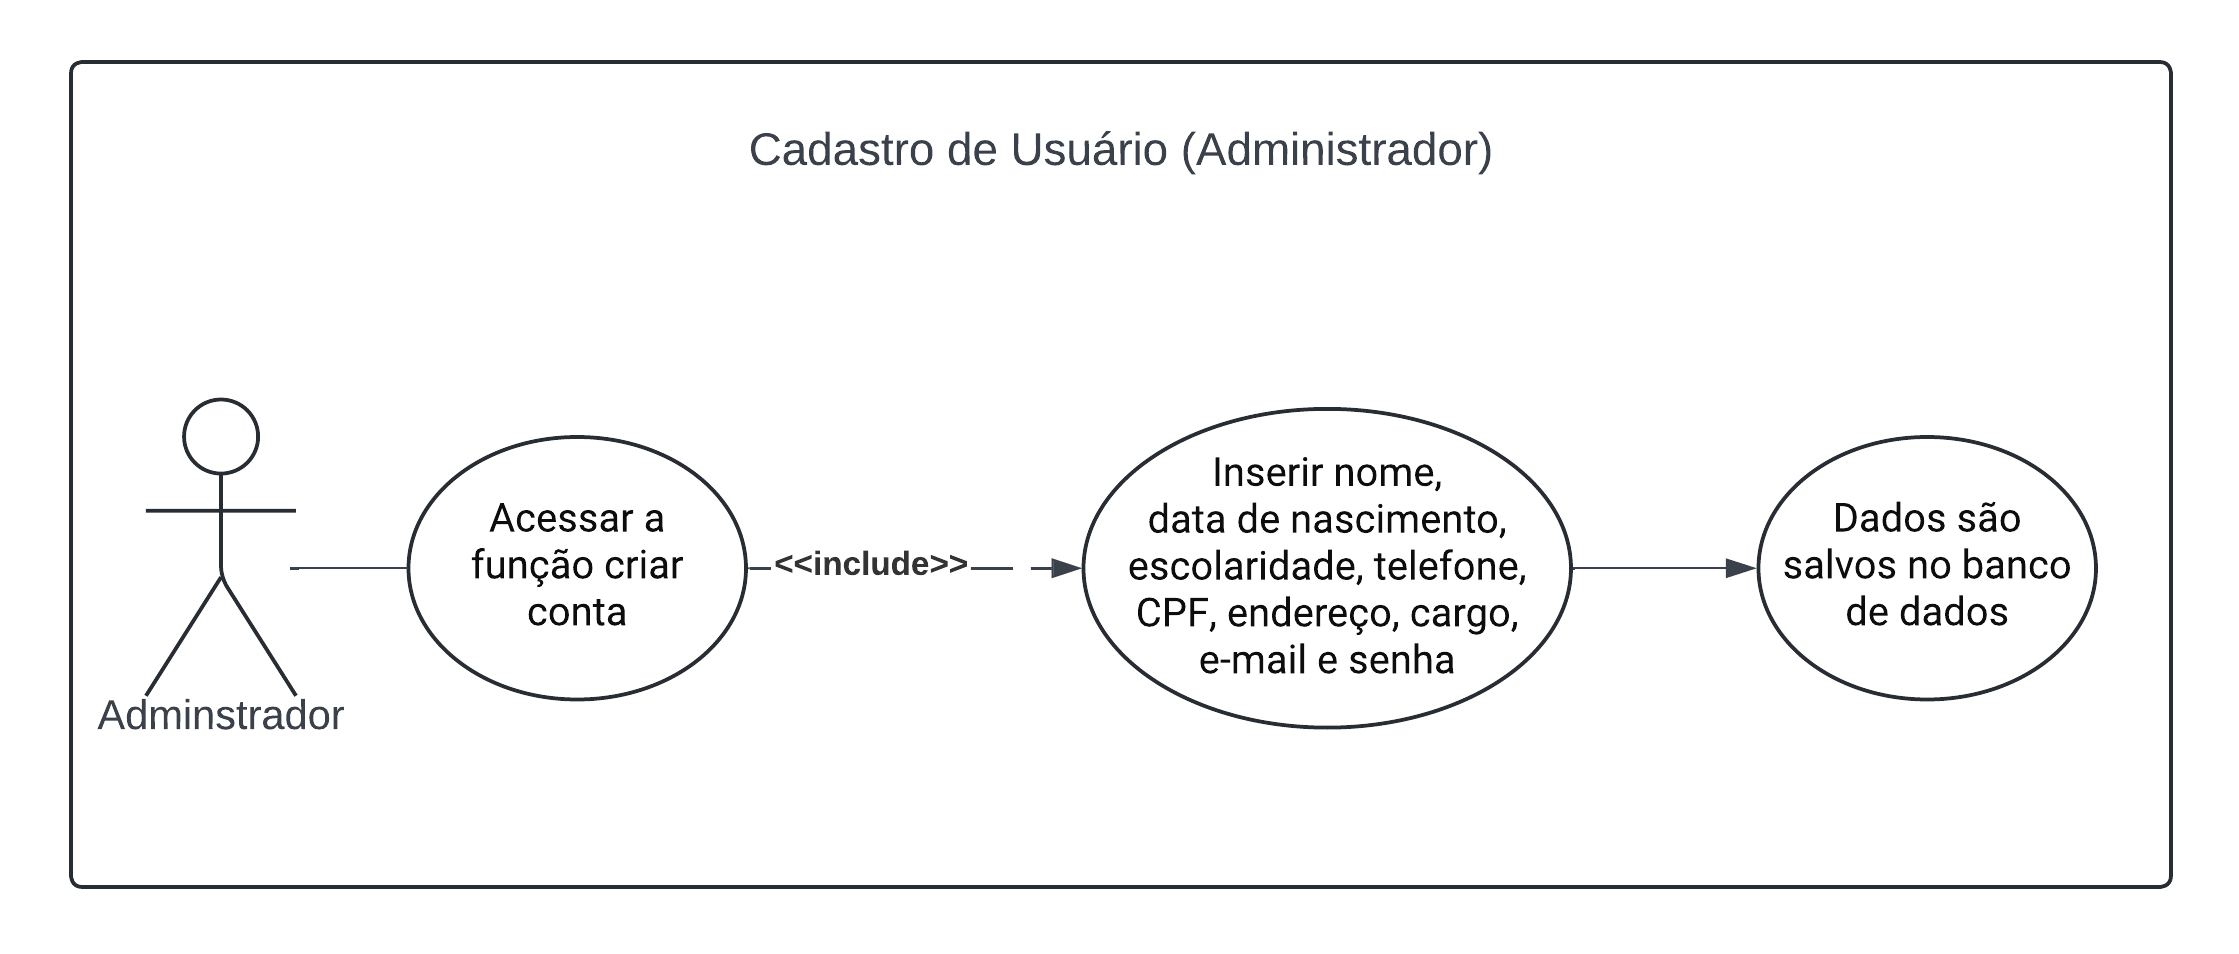
\includegraphics[scale=0.8]{caso-de-uso_cadastro-de-usuario-administrador.png}
            \caption{Caso de Uso: Cadastro de Usuário (Administrador)}
            \label{fig:enter-label}
        \end{figure}
        
        \begin{itemize}
            \item \textbf{Ator Principal:} Administrador
            \item \textbf{Interessados e Interesses:}
            
            O administrador deseja criar e gerenciar sua conta para acessar as funcionalidades de manutenção das perguntas do teste vocacional.
            \item \textbf{Pré-Condições:}
            
            O administrador possui permissão para ter um cadastro na plataforma.
             \item \textbf{Fluxo Básico:}

             \begin{itemize}
                 \item O administrador acessa a página de cadastro de administrador no sistema.
                 \item O sistema solicita ao administrador que insira seu nome, data de nascimento, escolaridade, telefone, CPF, endereço, cargo, e-mail e senha.
                 \item O administrador insere seus dados conforme o solicitado pelo sistema.
                 \item O sistema valida os dados inseridos pelo administrador.
                 \item O sistema verifica se o e-mail é único no sistema.
                 \item O sistema salva os dados do administrador no banco de dados.
                 \item O administrador recebe uma confirmação de que seu cadastro foi realizado com sucesso.
             \end{itemize}


            \item \textbf{Fluxos Alternativos:}
            \begin{itemize}
                \item Se o e-mail fornecido pelo administrador já estiver em uso, o sistema exibe uma mensagem de erro e solicita que o administrador insira um e-mail válido.
                \item Se o administrador inserir um e-mail inválido, o sistema exibirá uma mensagem de erro e solicitará que o administrador corrija o e-mail.
                \item Se o administrador inserir um CPF inválido, o sistema exibirá uma mensagem de erro e solicitará que o administrador corrija o CPF.
                \item Se o administrador não preencher todos os campos obrigatórios, o sistema exibirá uma mensagem de erro e solicitará que o administrador complete os campos em falta.
            \end{itemize}
            \item \textbf{Fluxo de Exceção:}
            \begin{itemize}
                \item O sistema enfrenta uma falha técnica:
                \begin{itemize}
                    \item O sistema exibe uma mensagem de erro informando sobre a falha técnica.
                    \item O caso de uso é encerrado.
                \end{itemize}
            \end{itemize}
        \end{itemize}
\end{itemize}

\begin{itemize}
    \item \textbf{Caso de Uso: Cadastro de Instituição Pública}

    \begin{figure}[ht]
        \centering
        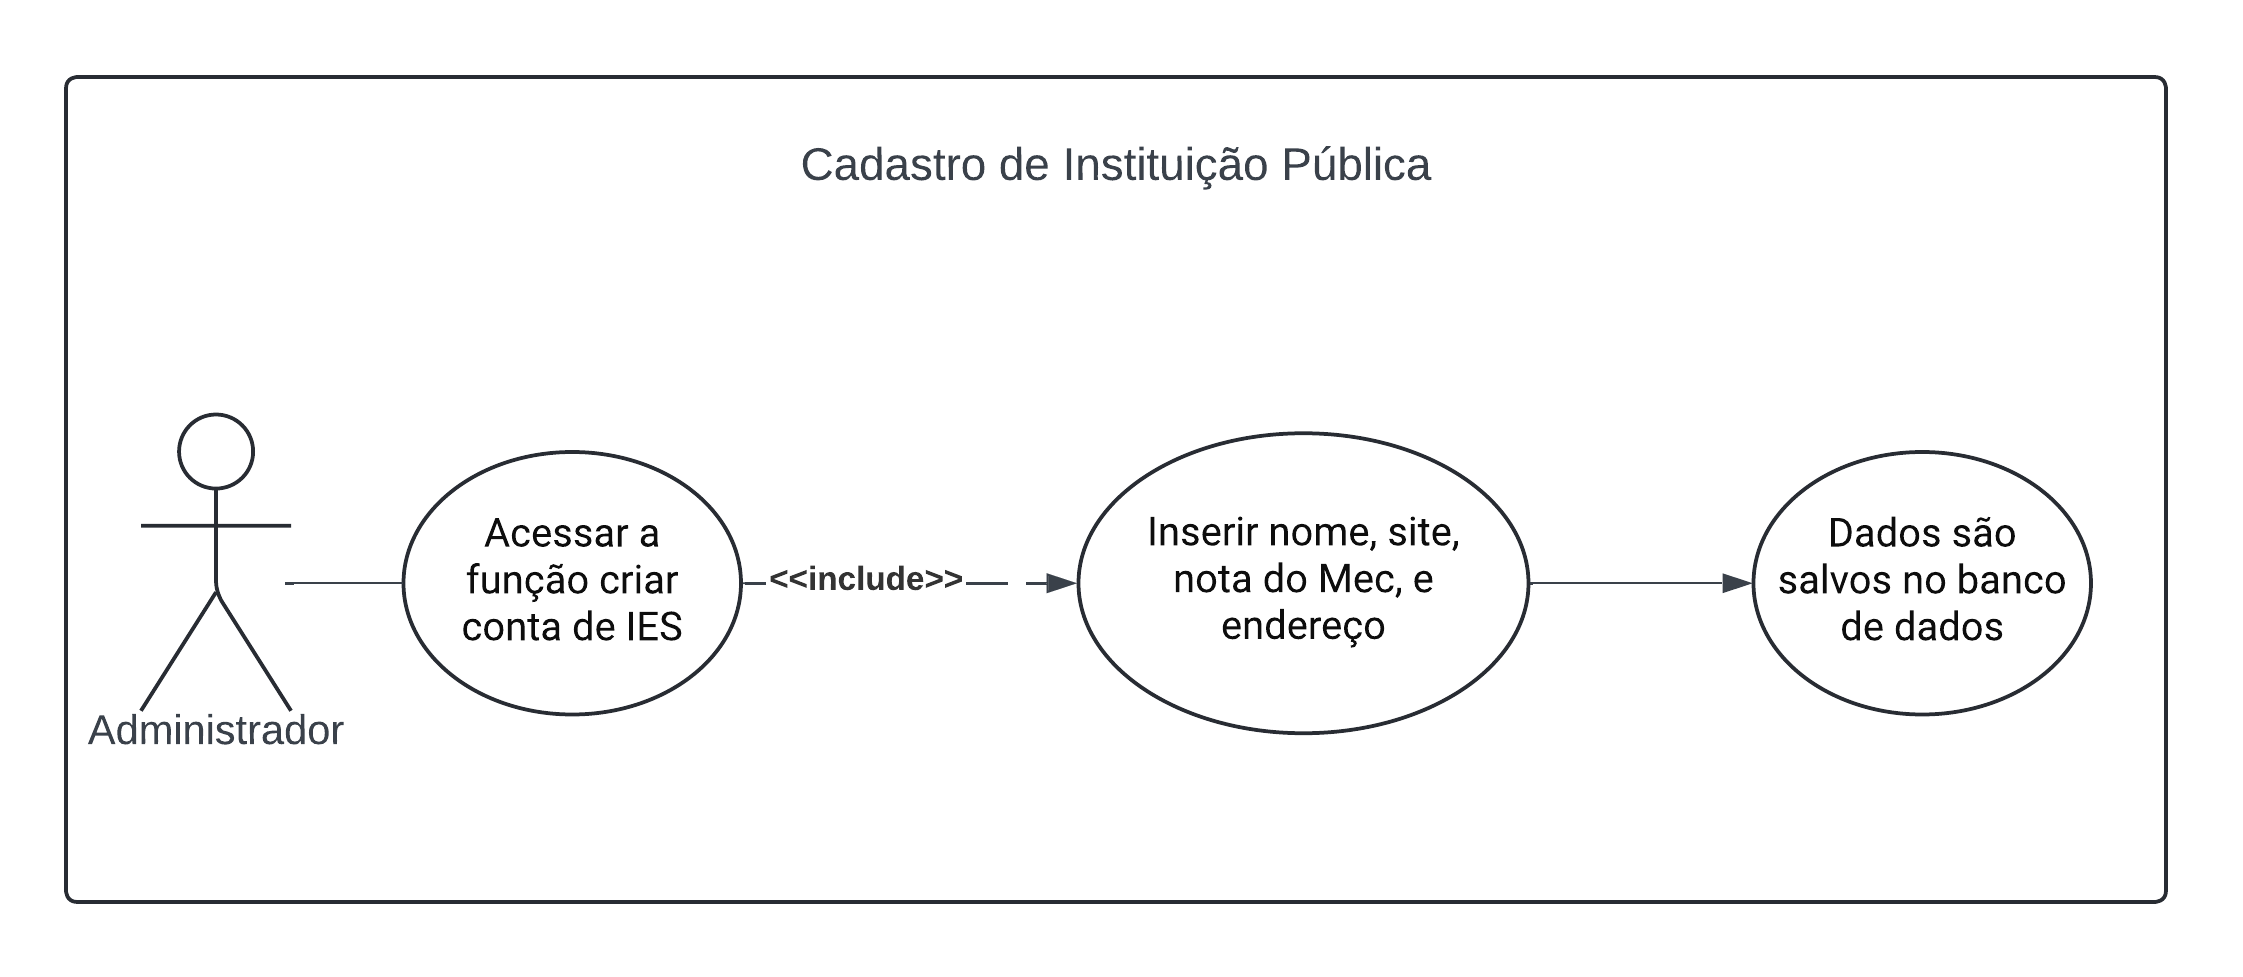
\includegraphics[scale=0.8]{caso-de-uso_cadastro-de-usuario-instituição.png}
        \caption{Caso de Uso: Cadastro de Instituição Pública}
        \label{fig:enter-label}
    \end{figure}

    \begin{itemize}
        \item \textbf{Ator Principal:}Administrador
        \item \textbf{Interessados e Interesses:}

        O Administrador deseja cadastrar uma instituição pública na plataforma para disponibilizar informações sobre seus cursos, formas de ingresso e políticas públicas de acesso e permanência.

        \item \textbf{Pré-Condições:}

        \item O Administrador possui cadastro na plataforma.
        \item A instituição pública possui as informações necessárias para o cadastro (nome, site, nota do Mec, endereço).
        \item \textbf{Fluxo Básico:}
        \begin{itemize}
            \item O administrador acessa a funcionalidade de cadastro de instituição na plataforma.
            \item O sistema solicita ao administrador que insira os dados da instituição pública, como nome da instituição, site da instituição, nota do MEC (Ministério da Educação) e endereço completo da instituição.
            \item O administrador preenche os campos obrigatórios com as informações solicitadas.
            \item O sistema verifica se os dados fornecidos são válidos e únicos no sistema.
            \item O sistema salva os dados da instituição pública no banco de dados.
            \item O administrador recebe uma confirmação de que a instituição pública foi cadastrada com sucesso.
        \end{itemize}
        \item \textbf{Fluxos Alternativos:}
        \begin{itemize}
            \item Se o administrador tentar cadastrar a instituição pública com um nome que já está em uso, o sistema exibirá uma mensagem de erro e solicitará um nome válido e único.
            \item Se o administrador tentar cadastrar a instituição pública com um site que não é válido, o sistema exibirá uma mensagem de erro e solicitará um site válido.
            \item Se o administrador tentar cadastrar a instituição pública com uma nota do MEC que não está dentro do intervalo válido, o sistema exibirá uma mensagem de erro e solicitará uma nota válida.
            \item Se o administrador tentar cadastrar a instituição pública com um endereço incompleto ou inválido, o sistema exibirá uma mensagem de erro e solicitará um endereço válido e completo.
        \end{itemize}
        \item \textbf{Fluxo de Exceção:}
        \begin{itemize}
            \item O sistema enfrenta uma falha técnica:
            \begin{itemize}
                \item O sistema exibe uma mensagem de erro informando sobre a falha técnica.
                \item O caso de uso é encerrado.
            \end{itemize}
        \end{itemize}
    \end{itemize}
\end{itemize}
\begin{itemize}
    \item \textbf{Caso de Uso: Cadastro de Usuário (Estudante)}

    \begin{figure}[ht]
        \centering
        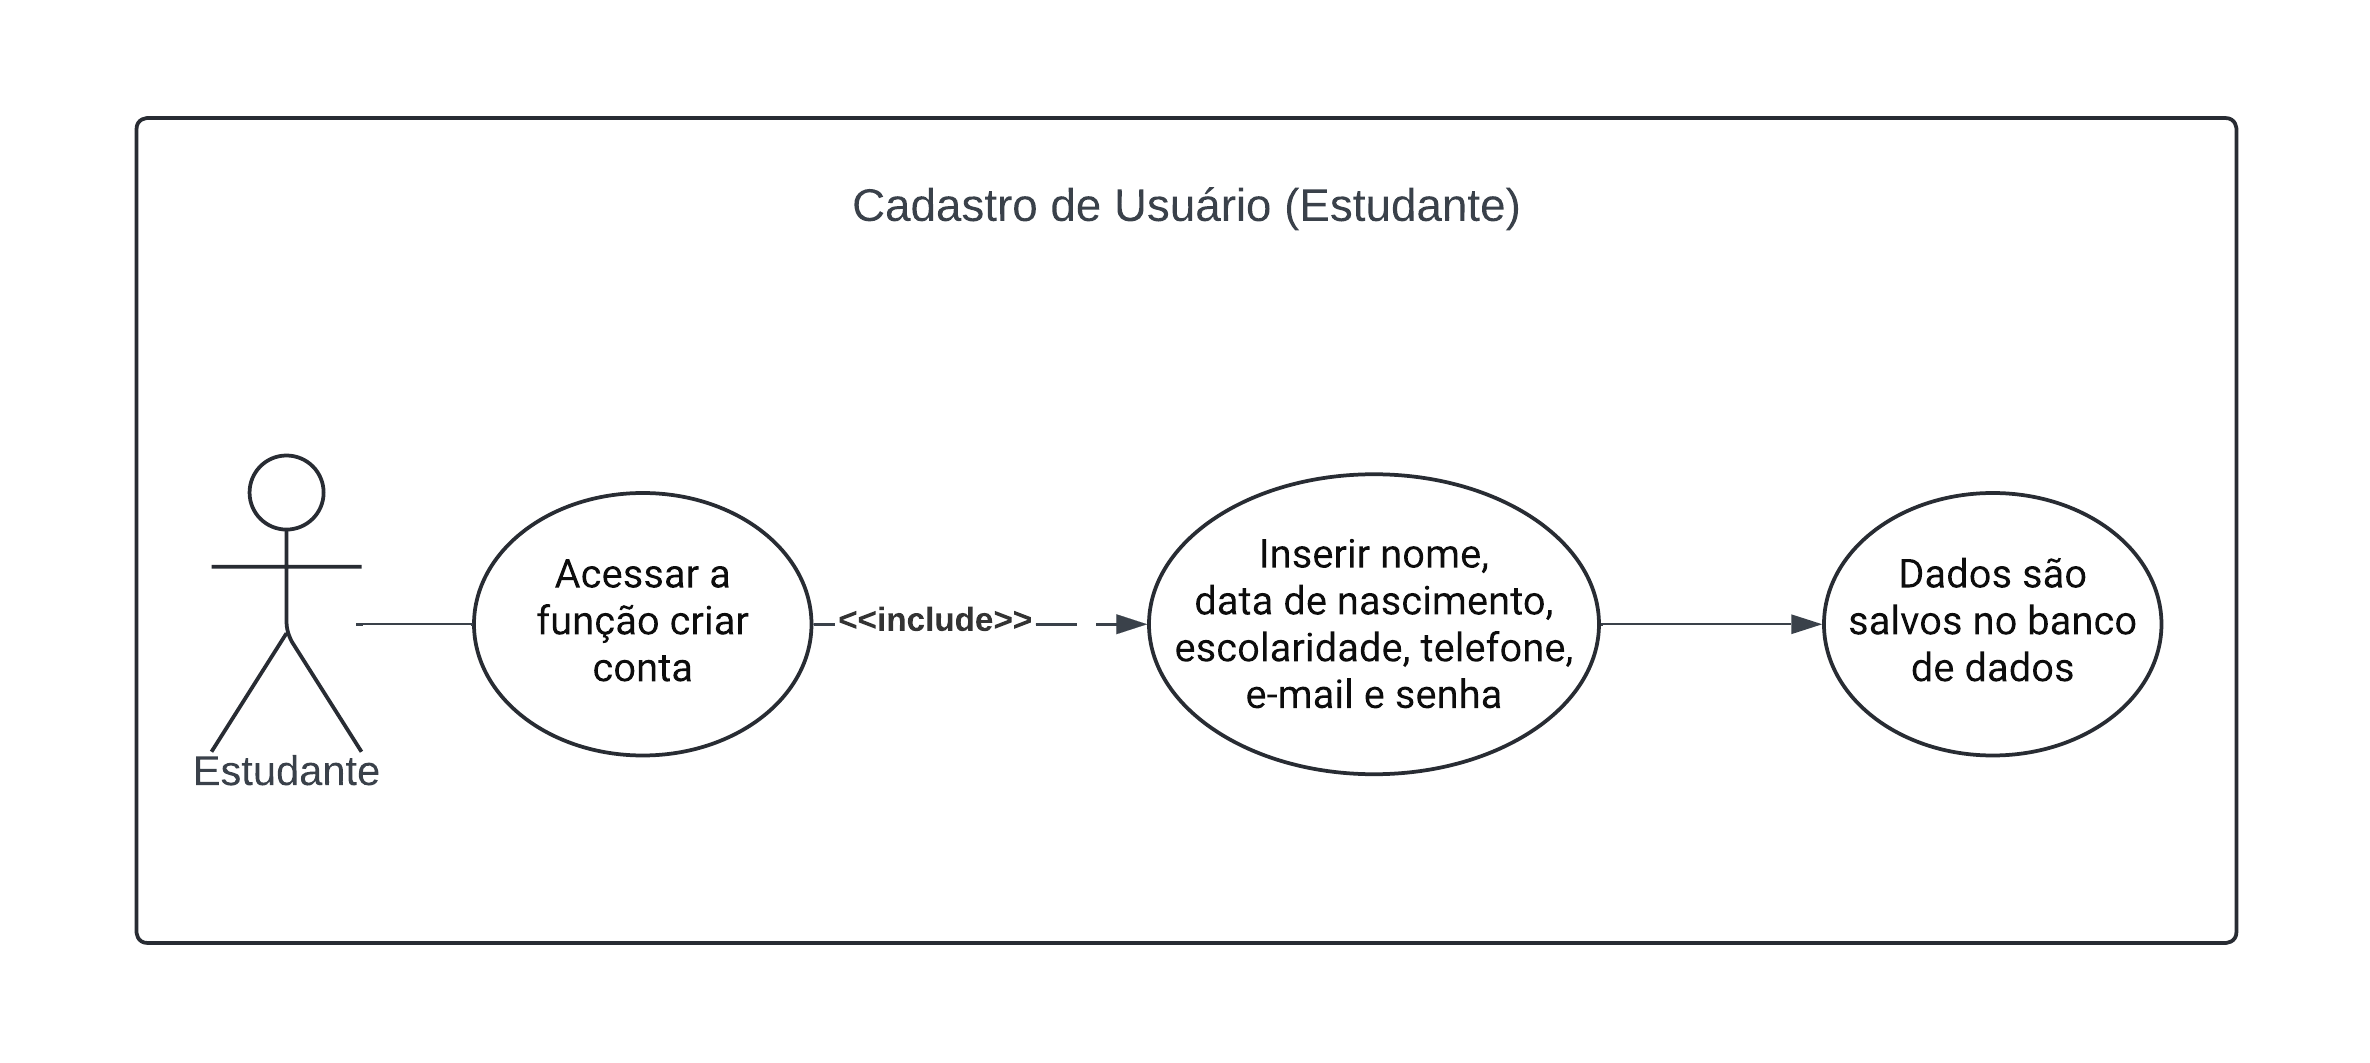
\includegraphics[scale=0.8]{caso-de-uso_cadastro-de-usuario-estudante.png}
        \caption{Caso de Uso: Cadastro de Usuário (Estudante)}
        \label{fig:enter-label}
    \end{figure}
    
    \begin{itemize}
        \item \textbf{Ator Principal:}Estudante.
        \item \textbf{Interessados e Interesses:}

        O estudante deseja se cadastrar na plataforma para ter acesso ao teste vocacional personalizado e às informações sobre as universidades públicas.

        \item \textbf{Pré-Condições:}

        O estudante possui mais de 14 anos de idade.
        \item \textbf{Fluxo Básico:}
        \begin{itemize}
            \item O estudante acessa a página de cadastro de usuário
            \item O sistema solicita ao estudante que preencha os campos obrigatórios, como nome, data de nascimento, escolaridade, telefone, e-mail e senha.
            \item O estudante preenche os campos obrigatórios.
            \item O sistema valida os dados inseridos pelo estudante.
            \item O sistema cria uma conta para o estudante e salva os dados no banco de dados.
            \item O estudante recebe uma confirmação de que seu cadastro foi realizado com sucesso.
        \end{itemize}
        \item  \textbf{Fluxos Alternativos:}
        \begin{itemize}
            \item Se o estudante inserir um e-mail inválido, o sistema exibirá uma mensagem de erro e solicitará que o estudante corrija o e-mail.
            \item Se o estudante não preencher todos os campos obrigatórios, o sistema exibirá uma mensagem de erro e solicitará que o estudante complete os campos em falta.
        \end{itemize}
        \item \textbf{Fluxo de Exceção:}
        \begin{itemize}
            \item O sistema enfrenta uma falha técnica:
            \begin{itemize}
                \item O sistema exibe uma mensagem de erro informando sobre a falha técnica.
                \item O caso de uso é encerrado.
            \end{itemize}
        \end{itemize}
    \end{itemize}
\end{itemize}
\begin{itemize}
    \item \textbf{Caso de Uso: Manter Perguntas do Teste Vocacional}
    
    \begin{figure}[ht]
        \centering
        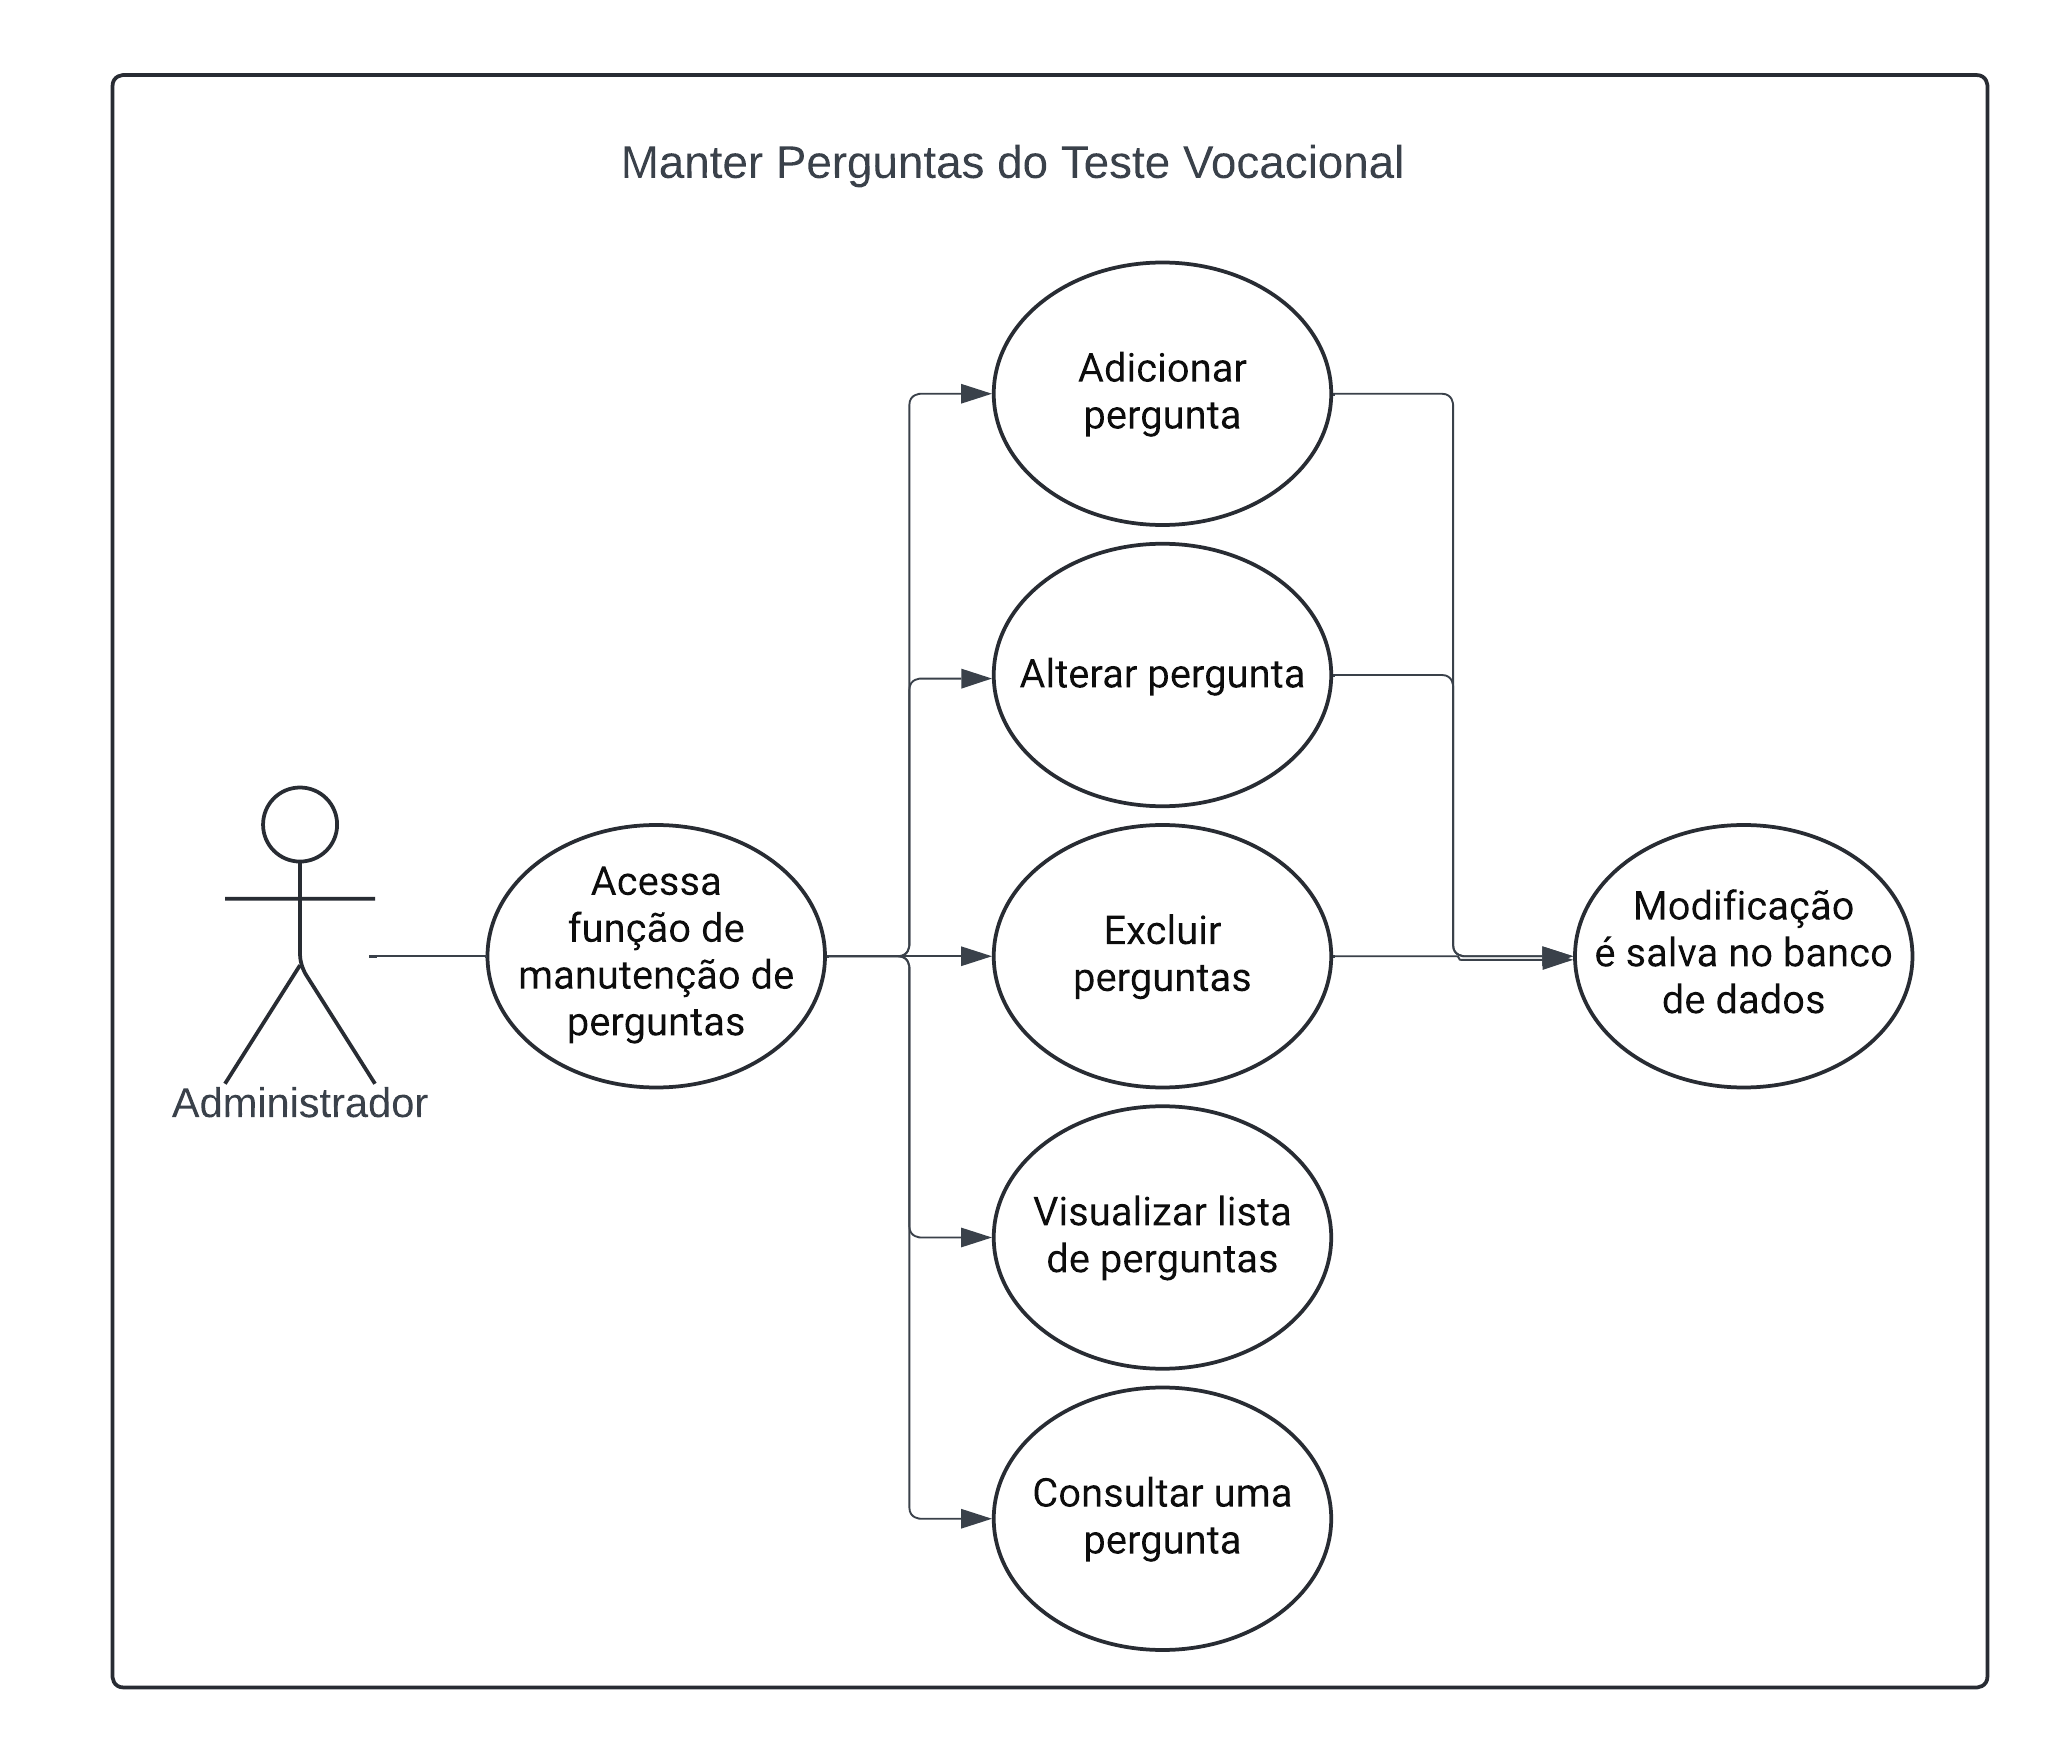
\includegraphics[scale=0.8]{caso-de-uso_manter-perguntas-do-teste-vocacional.png}
        \caption{Caso de Uso: Manter Perguntas do Teste Vocacional}
        \label{fig:enter-label}
    \end{figure}

    \begin{itemize}
        \item  \textbf{Ator Principal:}Administrador
        \item \textbf{Interessados e Interesses:}

        O administrador deseja gerenciar as perguntas do teste vocacional para garantir a qualidade e relevância do teste para os estudantes.
        \item \textbf{Pré-Condições:}
        \begin{itemize}
            \item O administrador possui acesso ao sistema.
            \item Para a funcionalidade de alterar e excluir perguntas, deve haver ao menos uma pergunta cadastrada no sistema.
        \end{itemize}
        \item \textbf{Fluxo Básico:}
        \begin{itemize}
            \item O administrador acessa a funcionalidade de manutenção de perguntas do teste vocacional.
            \item O sistema exibe a lista de perguntas existentes.
            \item O administrador escolhe entre incluir, alterar, excluir ou consultar uma pergunta.
            \begin{itemize}
                \item \textbf{Incluir Pergunta:}                
                \item O sistema solicita ao administrador que insira o texto da nova pergunta.
                \item O administrador insere o texto da pergunta.
                \item O sistema salva a nova pergunta no banco de dados.
                
                \item \textbf{Alterar Pergunta:}
                \item O sistema exibe as perguntas existentes e suas opções de edição.
                \item O administrador seleciona a pergunta que deseja modificar.
                \item O sistema permite que o administrador edite o texto da pergunta selecionada.
                \item O administrador faz as alterações desejadas.
                \item O sistema salva as alterações no texto da pergunta.
                
                \item \textbf{Excluir Pergunta:}
                \item O sistema exibe as perguntas existentes e suas opções de exclusão.
                \item O administrador seleciona a pergunta que deseja excluir.
                \item O sistema solicita confirmação para excluir a pergunta selecionada.
                \item O administrador confirma a exclusão da pergunta.
                \item O sistema define a pergunta como inativa no banco de dados.
                
                \item \textbf{Consultar Pergunta:}
                \item O sistema exibe as perguntas existentes e suas opções de consulta.
                \item O administrador seleciona a pergunta que deseja consultar.
                \item O sistema exibe as informações detalhadas da pergunta, como o texto da pergunta e seu ID.
            \end{itemize}
            
            \item O sistema executa a ação escolhida pelo administrador e retorna à lista de perguntas, atualizando-a conforme necessário.
        \end{itemize}
        \item \textbf{Fluxos Alternativos:}
        \begin{itemize}
            \item Se o administrador tentar incluir uma pergunta com texto vazio, o sistema exibirá uma mensagem de erro e não permitirá a inclusão.
            \item Se o administrador tentar alterar uma pergunta que não existe, o sistema exibirá uma mensagem de erro e não permitirá a alteração.
            \item Se o administrador tentar excluir uma pergunta que não existe, o sistema exibirá uma mensagem de erro e não permitirá a exclusão.
        \end{itemize}
        \item \textbf{Fluxo de Exceção:}
        \begin{itemize}
            \item O sistema enfrenta uma falha técnica:
            \begin{itemize}
                \item O sistema exibe uma mensagem de erro informando sobre a falha técnica.
                \item O caso de uso é encerrado.
            \end{itemize}
        \end{itemize}
        
    \end{itemize}
\end{itemize}
\begin{itemize}
    \item \textbf{Caso de Uso: Manter Informações sobre Cursos}

    \begin{figure}[ht]
        \centering
        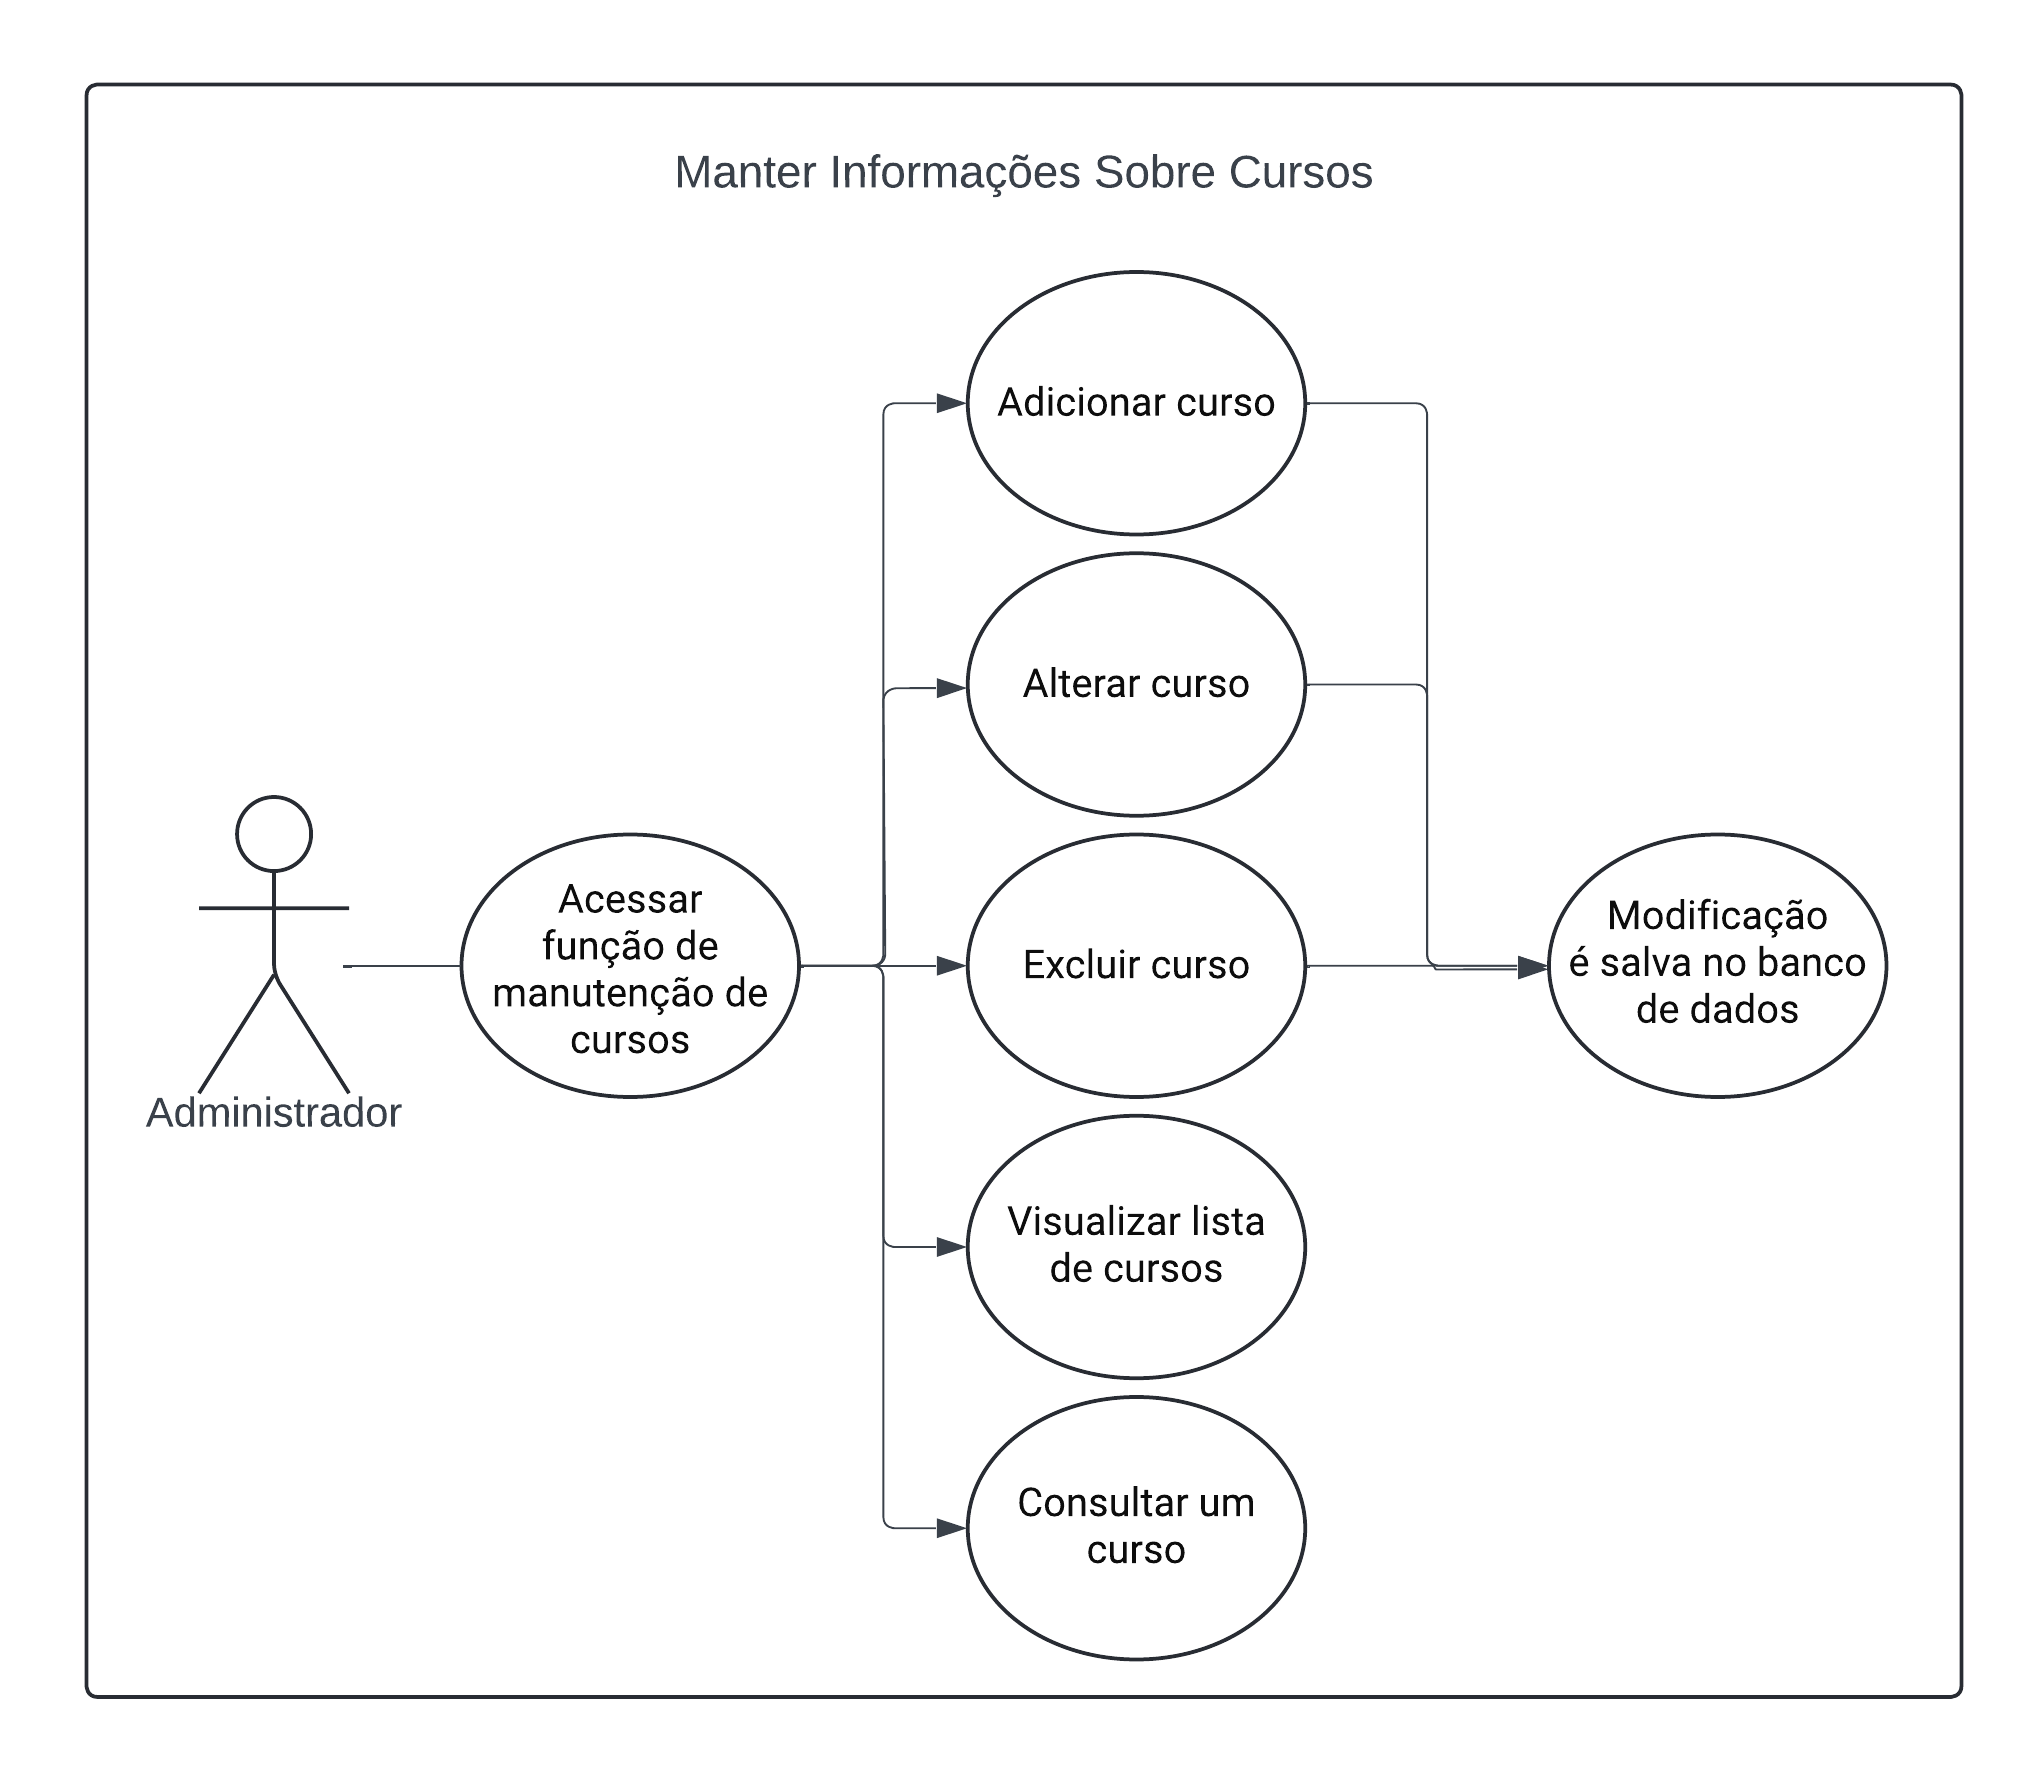
\includegraphics[scale=0.8]{caso-de-uso_manter-informações-sobre-cursos.png}
        \caption{Caso de Uso: Manter Informações sobre Cursos}
        \label{fig:enter-label}
    \end{figure}

    \begin{itemize}
        \item \textbf{Ator Principal:}Administrador.
        \item \textbf{Interessados e Interesses:}

        O administrador deseja manter informações atualizadas sobre os cursos oferecidos pela instituição pública na plataforma.
        \item \textbf{Pré-Condições:}
        \begin{itemize}
            \item O administrador possui acesso à plataforma de cadastro.
            \item A instituição pública já está devidamente cadastrada na plataforma.
        \end{itemize}
        \item \textbf{Fluxo Básico:}
        \begin{itemize}
            \item O administrador acessa a funcionalidade de manutenção de informações sobre cursos de uma instituição pública na plataforma.
            \item O sistema apresenta a lista de cursos cadastrados da instituição pública.
            \item  O administrador escolhe entre incluir, alterar, excluir ou consultar um curso.
            \begin{itemize}
                \item \textbf{Incluir Curso:}
                \item  O administrador insere os dados do novo curso, incluindo nome, descrição, grade curricular, formas de ingresso, empregabilidade, possiveis carreiras.
                \item O sistema valida os dados fornecidos pelo administrador.
                \item O sistema salva as informações do novo curso no banco de dados.
                \item \textbf{Alterar Curso:}
                \item  O administrador seleciona o curso que deseja alterar.
                \item O administrador faz as alterações necessárias nos dados do curso.
                \item O sistema valida as alterações feitas pelo administrador.
                \item O sistema salva as alterações no banco de dados.
                \item \textbf{Excluir Curso:}
                \item  O administrador seleciona o curso que deseja excluir.
                \item O sistema solicita confirmação para excluir o curso selecionado.
                \item  O administrador confirma a exclusão do curso.
                \item O sistema define o curso como inativo no banco de dados.
                \item \textbf{Consultar Curso:}
                \item  O administrador seleciona o curso que deseja consultar.
                \item O sistema exibe as informações detalhadas do curso selecionado.
                
            \end{itemize}
        \end{itemize}
        \item \textbf{Fluxos Alternativos:}
        \begin{itemize}
            \item Se  o administrador tentar incluir um curso com informações incompletas ou inválidas, o sistema exibirá uma mensagem de erro e solicitará informações válidas e completas.
            \item Se o administrador tentar alterar um curso que não existe, o sistema exibirá uma mensagem de erro e solicitará a seleção de um curso válido.
            \item Se  o administrador tentar excluir um curso que não existe, o sistema exibirá uma mensagem de erro e solicitará a seleção de um curso válido.
        \end{itemize}
        \item \textbf{Fluxo de Exceção:}
        \begin{itemize}
            \item O sistema enfrenta uma falha técnica:
            \begin{itemize}
                \item O sistema exibe uma mensagem de erro informando sobre a falha técnica.
                \item O caso de uso é encerrado.
            \end{itemize}
        \end{itemize}
        \item \textbf{Pós-Condições:}

        As informações sobre os cursos são atualizadas no sistema e podem ser consultadas pelos usuários da plataforma.
    \end{itemize}
\end{itemize}

\begin{itemize}
    \item \textbf{Caso de Uso: Responder o Teste Vocacional}

    \begin{figure}[ht]
        \centering
        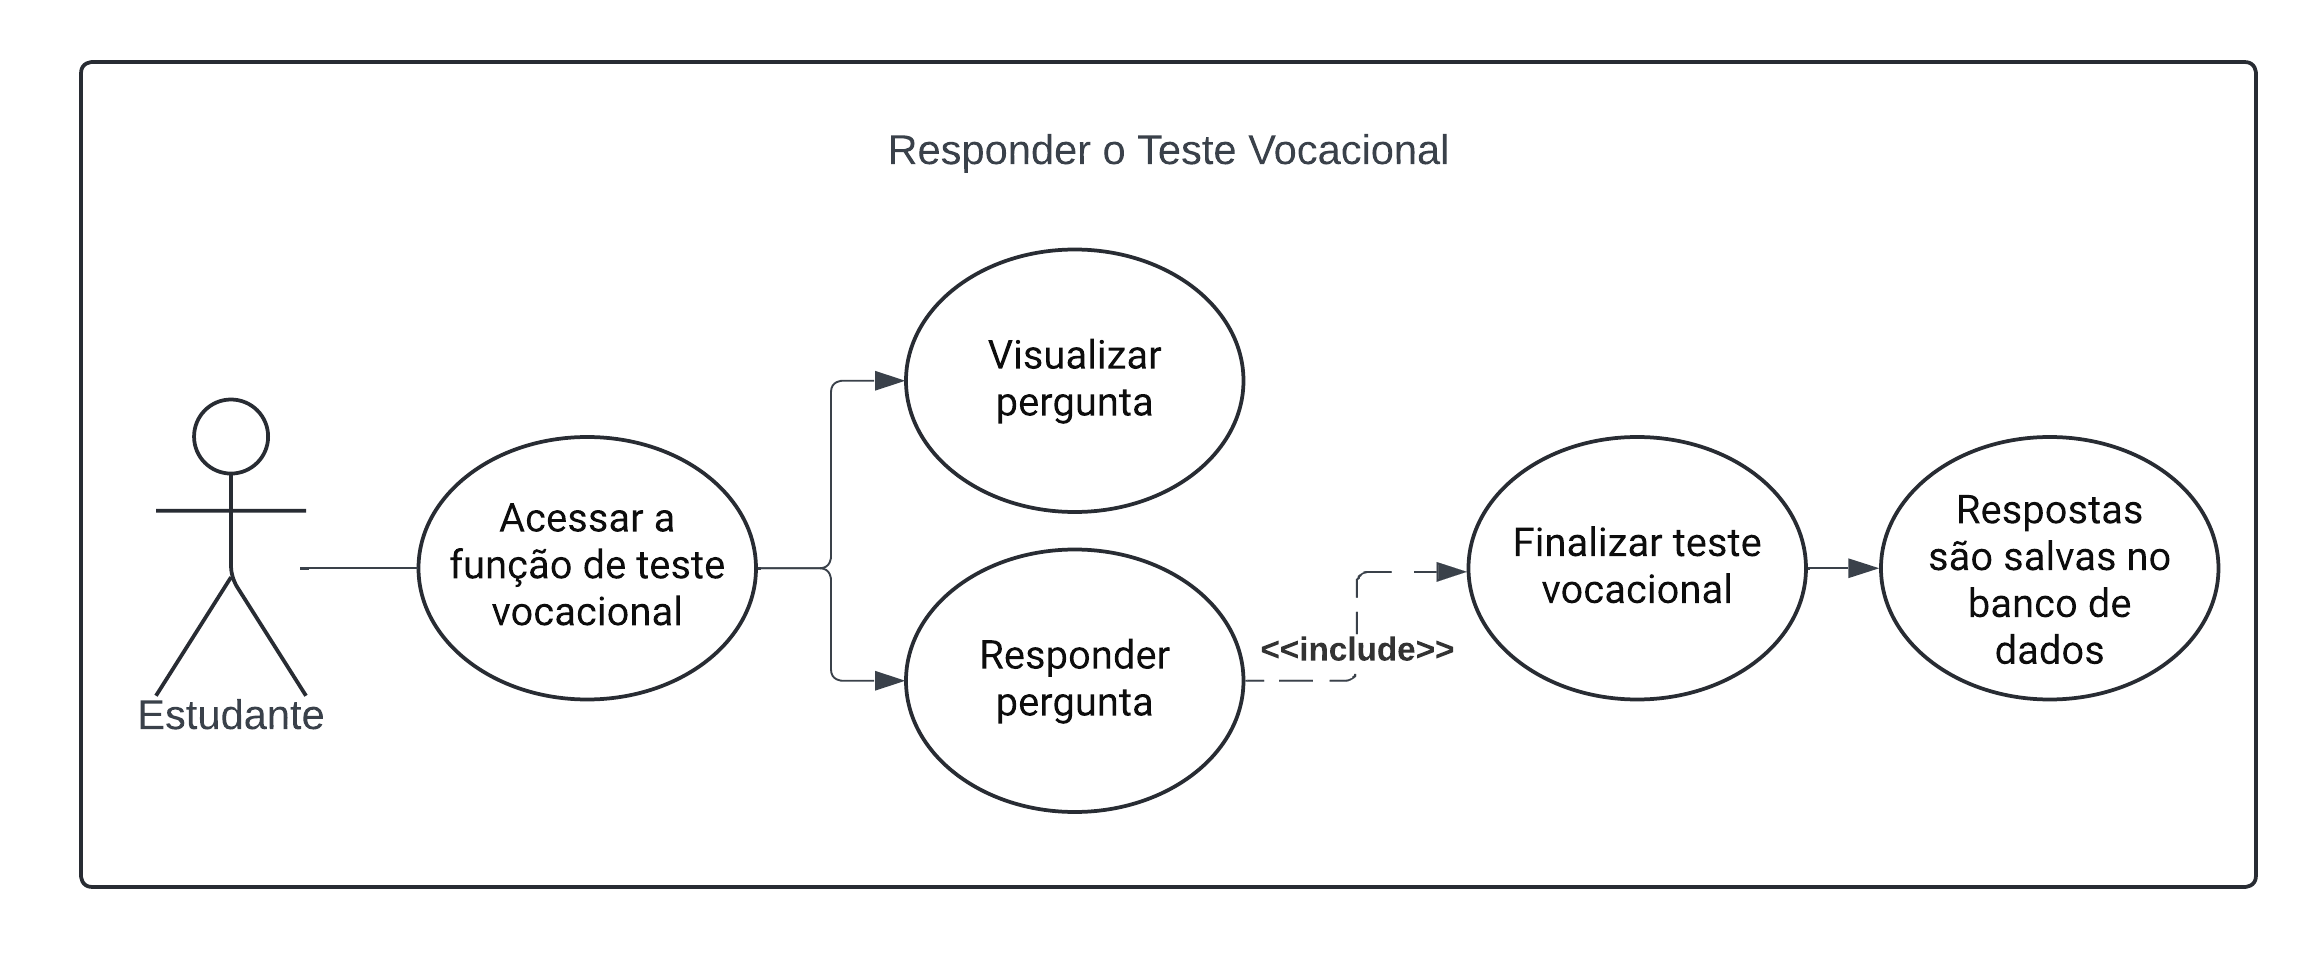
\includegraphics[scale=0.8]{caso-de-uso_responder-teste-vocacional.png}
        \caption{Caso de Uso: Responder o Teste Vocacional}
        \label{fig:enter-label}
    \end{figure}

    \item \textbf{Ator Principal:}Estudante
    \item \textbf{Interessados e Interesses:}

    Este caso de uso descreve como um estudante pode responder ao teste vocacional disponibilizado pela plataforma.
    \item \textbf{Pré-condições: }

    O estudante deve estar autenticado no sistema para acessar a funcionalidade de responder ao teste vocacional.
    \item \textbf{Fluxo Básico:}
    \begin{itemize}
        \item O estudante acessa a funcionalidade de responder ao teste vocacional no sistema.
        \item O sistema apresenta as perguntas do teste vocacional ao estudante.
        \item O estudante lê e responde às perguntas do teste de acordo com suas preferências e características.
        \item Após responder todas as perguntas, o estudante finaliza o teste.
        \item O sistema registra as respostas do estudante no banco de dados, associando-as ao perfil do estudante.
    \end{itemize}
    \item \textbf{Fluxos Alternativos:}
    \begin{itemize}
        \item Se o estudante interromper o teste antes de concluí-lo, o sistema preserva as respostas parciais registradas durante o teste, porém, somente as armazena no banco de dados após o estudante concluir integralmente o teste.
    \end{itemize}
    \item \textbf{Fluxo de Exceção:}
    \begin{itemize}
        \item Se o sistema enfrentar uma falha técnica durante o teste:
        \begin{itemize}
            \item O sistema exibe uma mensagem de erro informando sobre a falha técnica.
            \item O estudante pode tentar responder ao teste novamente após a resolução do problema técnico.
        \end{itemize}
    \end{itemize}
    \item \textbf{Pós-condições:}

    As respostas do estudante são registradas no sistema e podem ser utilizadas para gerar recomendações de cursos com base nos resultados do teste.
\end{itemize}

\begin{itemize}
    \item \textbf{Caso de Uso: Apresentar Recomendação de Curso}

    \begin{figure}[ht]
        \centering
        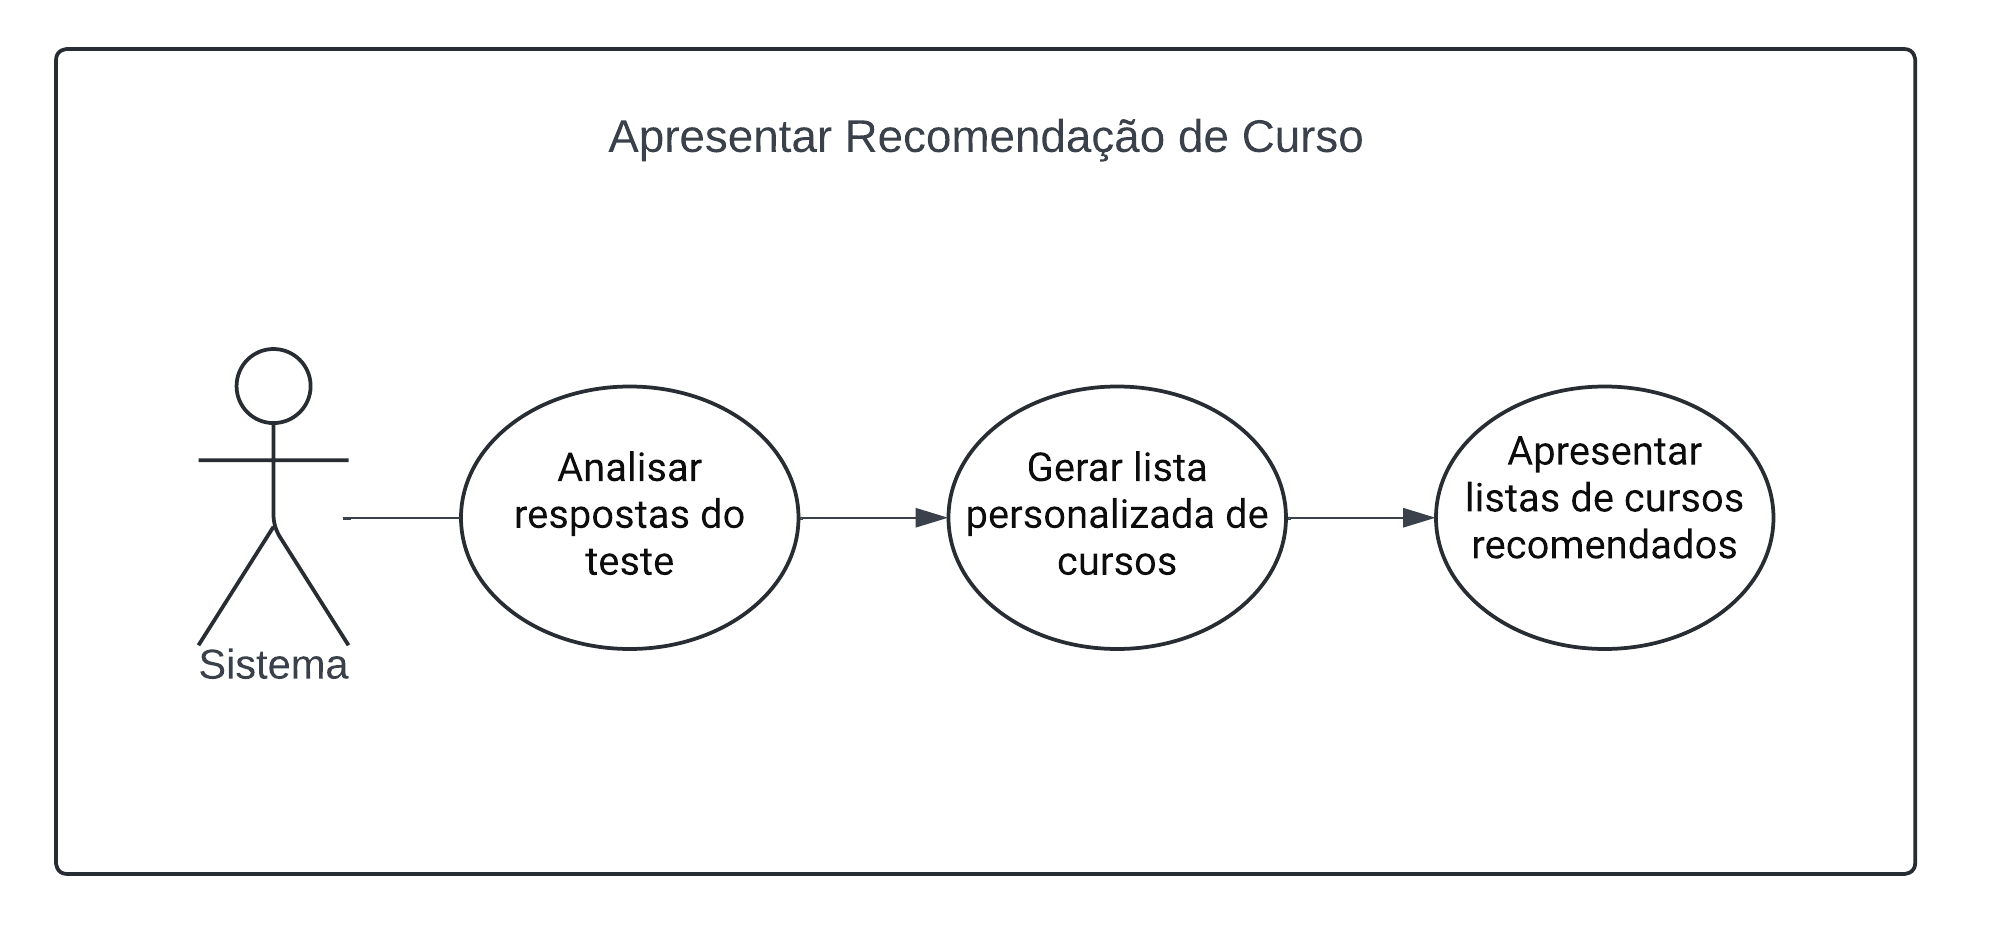
\includegraphics[scale=0.8]{caso-de-uso_recomendar-curso.png}
        \caption{Caso de Uso: Apresentar Recomendação de Curso}
        \label{fig:enter-label}
    \end{figure}
    \begin{itemize}
        \item \textbf{Ator Principal:}Sistema
        \item \textbf{Interessados e Interesses:}

        O sistema precisa fornecer uma recomendação personalizada de cursos para o estudante com base nas respostas do teste vocacional, auxiliando-o na escolha de sua formação acadêmica.
        \item \textbf{Pré-Condições:}
        \begin{itemize}
            \item O estudante realizou o teste vocacional e suas respostas estão registradas no sistema.
            \item O sistema possui algoritmos de análise e recomendação de cursos configurados.
        \end{itemize}
        \item \textbf{Fluxo Básico:}
        \begin{itemize}
            \item O sistema analisa as respostas do teste vocacional do estudante, que estão previamente registradas e associadas no banco de dados.
            \item Com base nas respostas analisadas, o sistema utiliza um algoritmo de recomendação para gerar uma lista de cursos que são mais adequados ao perfil do estudante.
            \item O sistema apresenta a lista de cursos recomendados ao estudante após a conclusão do teste vocacional.
        \end{itemize}
        \item \textbf{Fluxos Alternativos:}

        Se o sistema não conseguir gerar uma recomendação com base nas respostas do teste, ele pode sugerir ao estudante que procure orientação adicional de um orientador educacional.
        \item \textbf{Fluxo de Exceção:}
        \begin{itemize}
            \item O sistema enfrenta uma falha técnica ao gerar a recomendação de curso:
            \begin{itemize}
                \item O sistema exibe uma mensagem de erro informando sobre a falha técnica.
                \item O caso de uso é encerrado.
            \end{itemize}
        \end{itemize}
        \item \textbf{Pós-Condições:}

        O estudante recebe uma recomendação personalizada de cursos com base nas respostas do teste vocacional, auxiliando-o na escolha de sua formação acadêmica.
    \end{itemize}
\end{itemize}
\begin{itemize}
    \item \textbf{Caso de Uso: Consultar Informações das Instituições de Ensino Superior (IES)}

    \begin{figure}[ht]
        \centering
        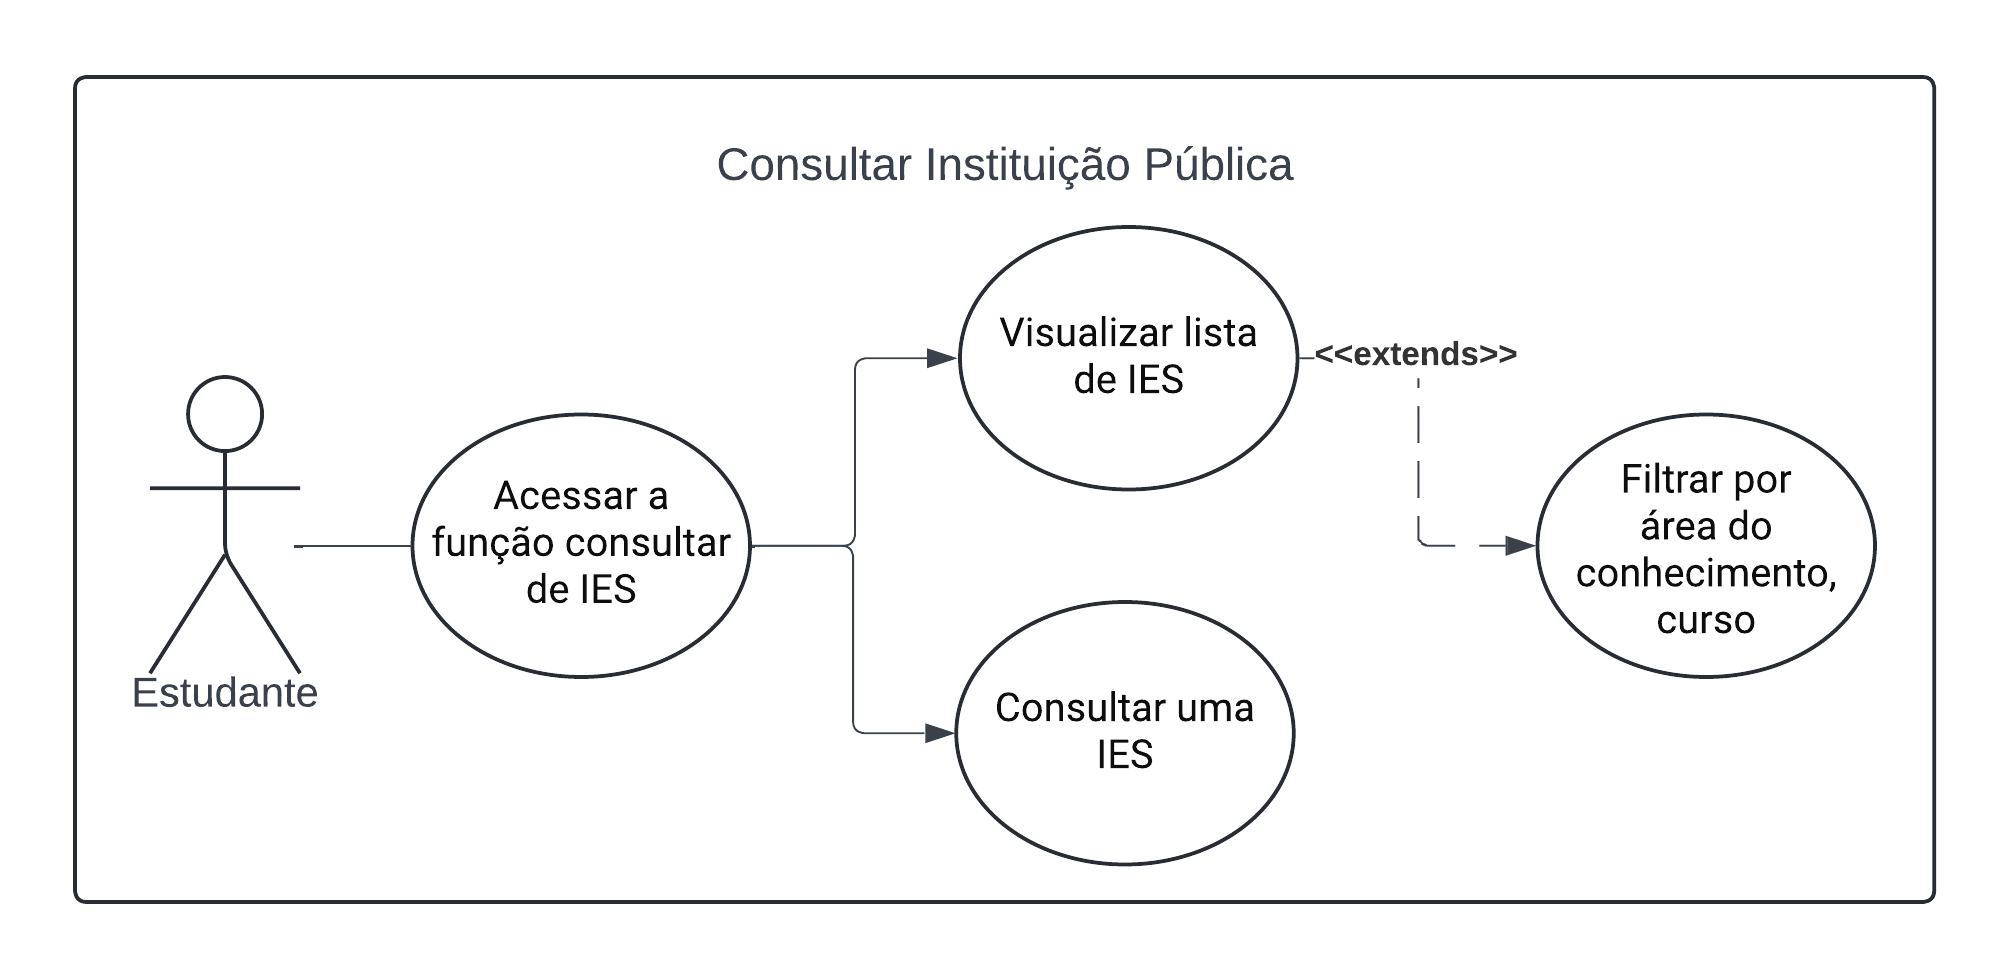
\includegraphics[scale=0.8]{caso-de-uso_consultar-ies.png}
        \caption{Caso de Uso: Consultar Informações das Instituições de Ensino Superior (IES)}
        \label{fig:enter-label}
    \end{figure}

    \begin{itemize}
        \item \textbf{Ator Principal:}Estudante
        \item \textbf{Interessados e Interesses:}

        O estudante deseja obter informações detalhadas sobre os cursos oferecidos pelas Instituições de Ensino Superior (IES) cadastradas na plataforma, permitindo filtrar as informações para encontrar cursos de seu interesse.

        \item \textbf{Pré-Condições:}  
        \begin{itemize}
            \item O estudante possui acesso à plataforma.
            \item As informações sobre os cursos e IES estão cadastradas e atualizadas na plataforma.
        \end{itemize}
        \item \textbf{Fluxo Básico:}
        \begin{itemize}
            \item O estudante acessa a funcionalidade de consultar informações sobre os cursos e IES na plataforma.
            \item O sistema exibe uma lista de cursos e IES cadastradas, apresentando informações básicas como nome do curso, nome da instituição, endereço, entre outras.
            \item O estudante pode utilizar filtros disponíveis na plataforma para refinar a busca, como por área de conhecimento, nome de curso, entre outros.
            \item O sistema atualiza dinamicamente a lista de cursos e IES conforme os filtros selecionados pelo estudante.
            \item O estudante visualiza as informações detalhadas dos cursos e IES selecionados na lista, incluindo grade curricular, notas de corte, empregabilidade, possiveis carreiras, entre outros detalhes relevantes.
        \end{itemize}
        \item  \textbf{Fluxos Alternativos:}

        Se não houver cursos ou IES cadastradas que correspondam aos critérios de busca do estudante, o sistema exibirá uma mensagem informando que não foram encontrados resultados.
        \item \textbf{Fluxo de Exceção:}
        \begin{itemize}
            \item O sistema enfrenta uma falha técnica ao gerar a recomendação de curso:
            \begin{itemize}
                \item O sistema exibe uma mensagem de erro informando sobre a falha técnica.
                \item O caso de uso é encerrado.
            \end{itemize}
        \end{itemize}
    \end{itemize}
\end{itemize}

\section{Arquitetura}

Nesse projeto, adotamos a \textbf{Clean Architecture} como o princípio norteador para o desenvolvimento do software. A decisão de seguir essa abordagem se fundamenta na necessidade de construir um sistema flexível e facilmente manutenível ao longo do tempo. Ao adotar a Clean Architecture, priorizamos a separação clara e bem definida das responsabilidades em diferentes camadas, como a de entidades de negócio, casos de uso, interfaces de usuário e infraestrutura. Isso não apenas promove uma estrutura organizada e modular, mas também facilita a realização de testes automatizados em cada uma dessas camadas, garantindo a qualidade do código e a detecção precoce de possíveis problemas. Além disso, ao desacoplar as regras de negócio das tecnologias específicas, tornamos o sistema mais adaptável a mudanças futuras, permitindo a evolução contínua do software de forma sustentável. 
\subsection{Back-End}
No que diz respeito ao back-end, adotamos o framework \textbf{Spring Boot} em conjunto com a arquitetura MSC (Model-Service-Controller). O Spring Boot é uma escolha popular para o desenvolvimento de aplicativos Java devido à sua facilidade de configuração e rápida inicialização. A arquitetura MSC divide a aplicação em três camadas distintas: \textbf{Model}, onde definimos as entidades e regras de negócio; \textbf{Service}, responsável pela lógica de negócio e manipulação dos dados; e \textbf{Controller}, que recebe as requisições HTTP e coordena a interação entre o cliente e o servidor. 

Além das camadas Model, Service e Controller, também implementamos a camada \textbf{Repository} como parte da arquitetura MSC. A camada Repository é responsável pela interação com o banco de dados, encapsulando a lógica de acesso e manipulação dos dados. Utilizando interfaces e métodos específicos, o Repository abstrai as operações CRUD (Create, Read, Update, Delete), permitindo que as demais camadas da aplicação interajam com o banco de dados de forma desacoplada e eficiente.

A utilização da arquitetura em camadas proporcionou diversos benefícios para o projeto. Em primeiro lugar, a separação de responsabilidades entre as camadas Model, Service, Controller e Repository facilitou a organização e compreensão do código-fonte, tornando-o mais legível e manutenível. Cada camada possui um propósito claro e bem definido, o que simplifica o processo de desenvolvimento e permite que diferentes equipes ou desenvolvedores trabalhem de forma independente em áreas específicas da aplicação.

\subsubsection{Gerenciamento de depêndencias}
Para o gerenciamento de dependências do projeto, optamos pelo \textbf{Maven}. Esta escolha se baseia nos inúmeros benefícios oferecidos por essa ferramenta. O Maven simplifica a gestão de dependências, permitindo que as bibliotecas necessárias sejam facilmente adicionadas ao projeto através de seu arquivo de configuração padrão (pom.xml). Além disso, o Maven automatiza tarefas como compilação, empacotamento e distribuição do projeto, tornando o processo de desenvolvimento mais eficiente e menos propenso a erros. Sua vasta gama de plugins oferece funcionalidades adicionais, como integração com ferramentas de teste e análise de código, promovendo uma abordagem mais completa para o desenvolvimento de software. 

\subsection{Front-End}
Nesse projeto, optamos por utilizar \textbf{React} em conjunto com \textbf{TypeScript} para o desenvolvimento do front-end. Essa escolha foi motivada pela necessidade de construir uma interface de usuário dinâmica e reativa, com uma base de código robusta e escalável. React é uma biblioteca JavaScript amplamente adotada que nos permite criar componentes reutilizáveis e composicionais, facilitando a construção de interfaces complexas de forma modular. Além disso, a integração com TypeScript adiciona um sistema de tipos estáticos ao JavaScript, oferecendo benefícios como detecção de erros em tempo de compilação e melhorando a manutenibilidade do código. A arquitetura baseada em componentes nos permitiu organizar a aplicação de forma hierárquica, facilitando a manutenção e o teste dos diferentes elementos da interface.
 
\subsection{Banco de dados}
Em relação ao banco de dados,  optamos pelo \textbf{MySQL} devido à sua confiabilidade, desempenho e ampla adoção na indústria. O MySQL é um sistema de gerenciamento de banco de dados relacional que oferece recursos avançados de segurança e escalabilidade, sendo uma escolha sólida para aplicações de diferentes tamanhos e complexidades. Utilizamos o MySQL para armazenar e gerenciar os dados da aplicação, garantindo a integridade e disponibilidade das informações.

\subsubsection{Modelo Entidade Relacionamento}
\begin{figure}[ht]
        \centering
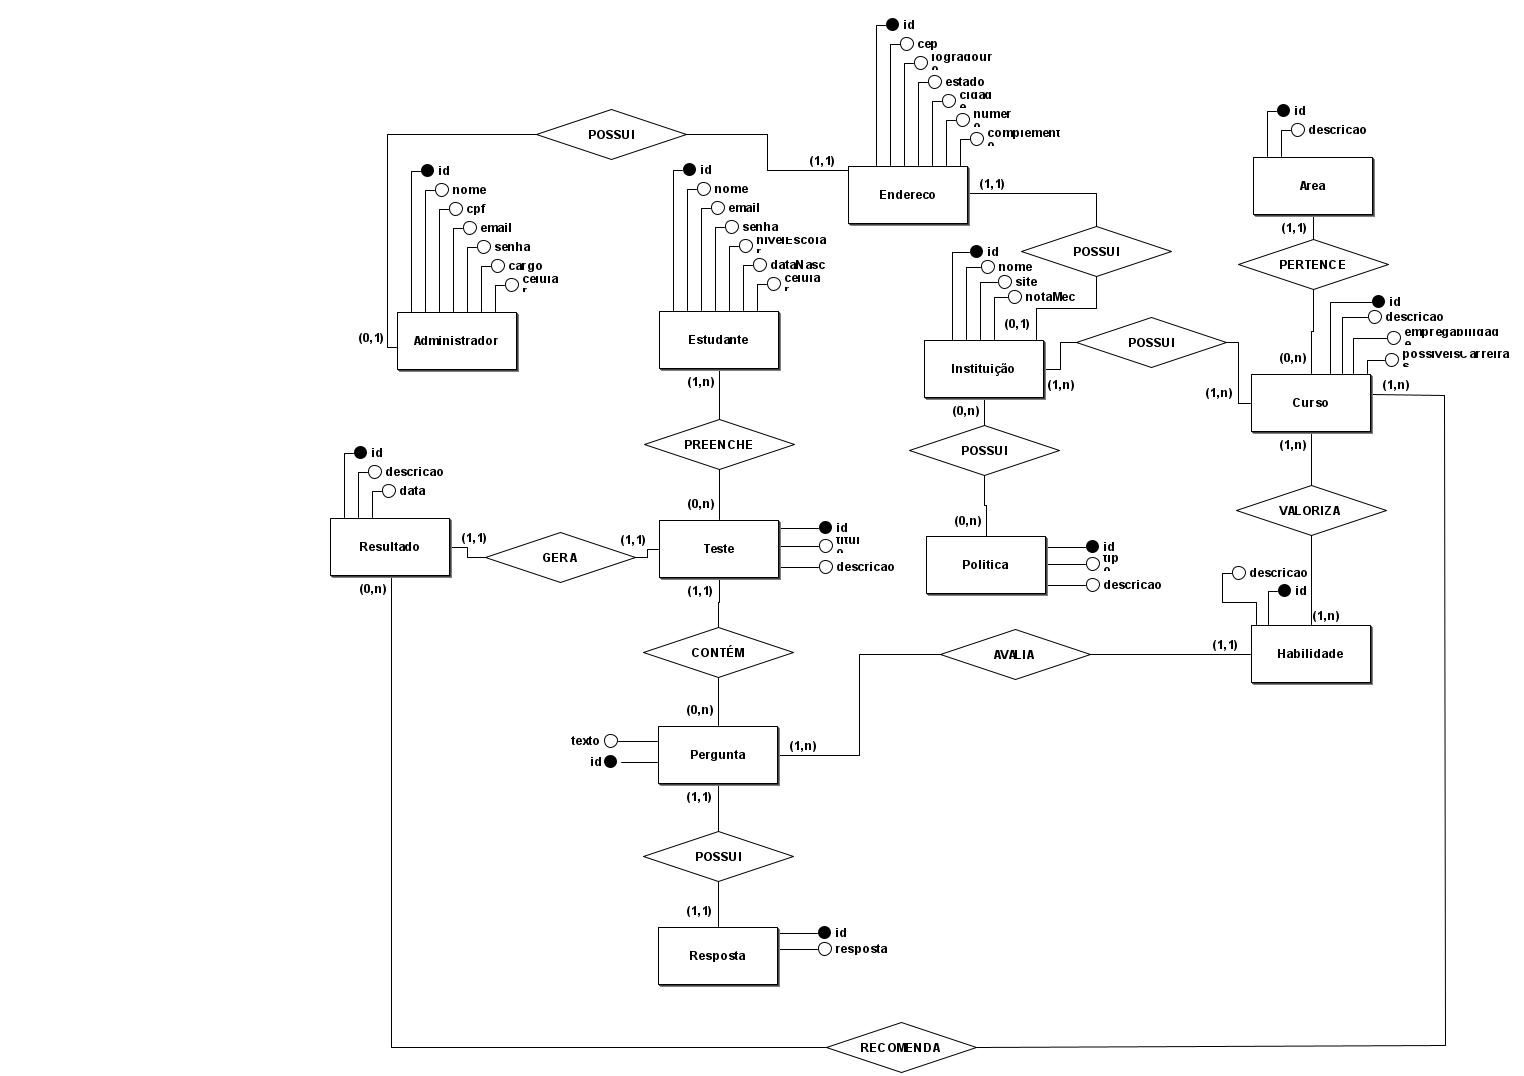
\includegraphics[width=0.8\textwidth]{mer.png}
        \caption{Modelo Entidade Relacionamento (MER) do projeto}
        \label{fig:enter-label}
    \end{figure}
    
\subsubsection{Diagrama Entidade Relacionamento}
\begin{figure}[ht]
        \centering
        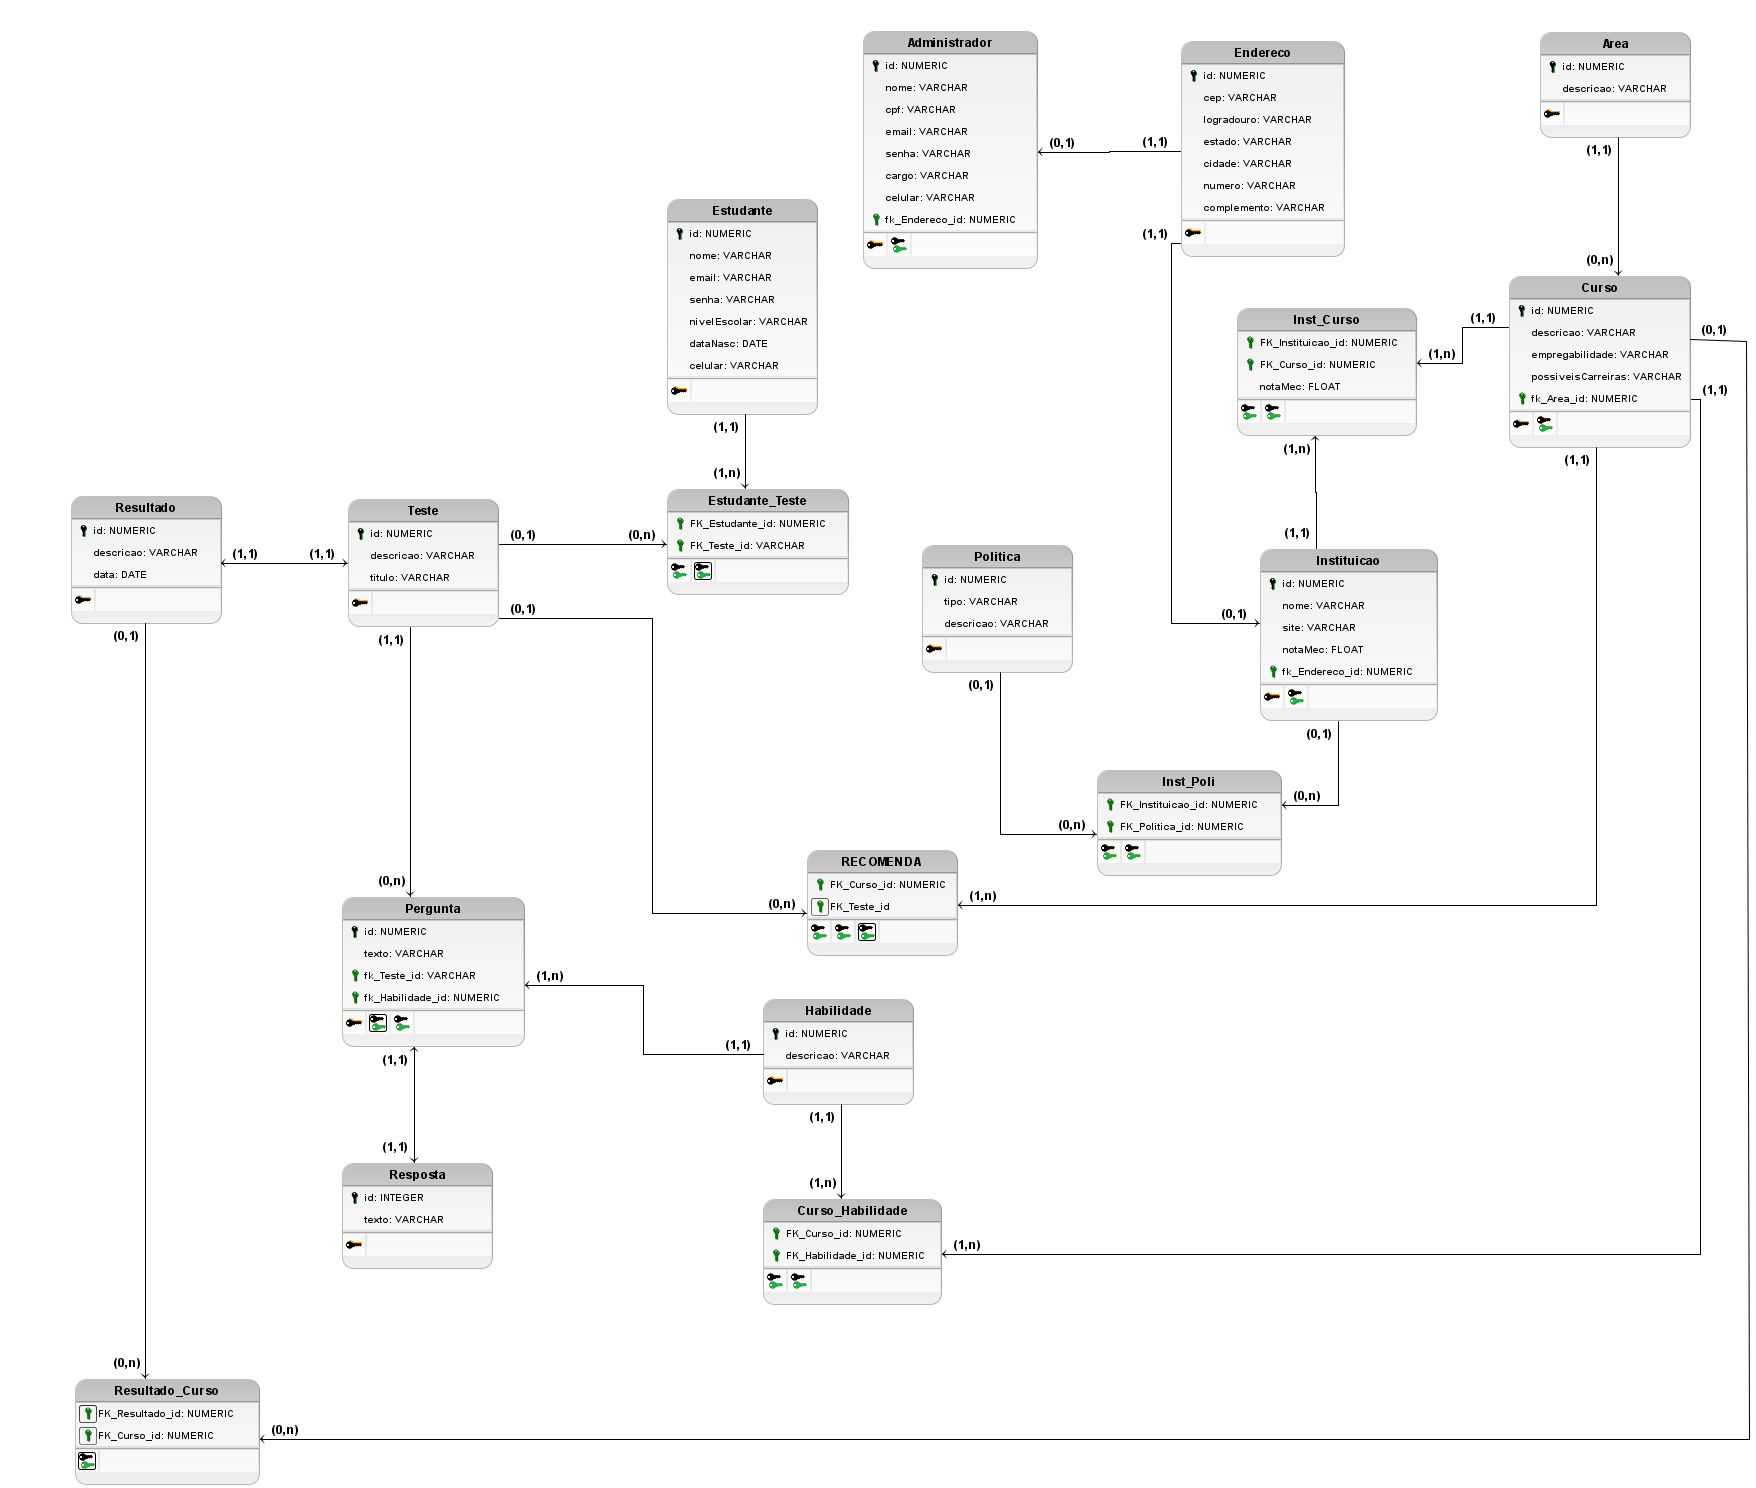
\includegraphics[width=1.0\textwidth]{modeloLogico.png}
        \caption{Diagrama Entidade Relacionamento (DER) do projeto}
        \label{fig:enter-label}
    \end{figure}


\subsection{Integrações}
Para aprimorar a experiência do usuário e garantir a precisão dos dados de endereço nos cadastros, optamos por integrar a API do \textbf{ViaCEP}. Essa integração permite que, ao preencher os campos de endereço em formulários de cadastro, o sistema automaticamente consulte a API do ViaCEP para obter informações detalhadas, como rua, bairro, cidade e estado, com base no CEP fornecido pelo usuário. Essa abordagem simplifica e agiliza o processo de preenchimento dos cadastros, além de garantir a consistência e atualização dos dados de endereço. Ao utilizar essa API, estamos priorizando a precisão e a eficiência na coleta e manipulação das informações de endereço, proporcionando uma experiência mais fluida e intuitiva para os usuários.
\subsection{Infraestrutura}
Por fim, para hospedar nosso projeto, escolhemos a plataforma \textbf{Railway}. A Railway oferece uma solução conveniente e eficiente para implantar e gerenciar aplicativos web, com integração contínua e implantação contínua que simplificam o processo de desenvolvimento e garantem entregas rápidas e seguras. Além disso, a plataforma oferece recursos de escalabilidade automática e monitoramento de desempenho, garantindo uma experiência confiável para os usuários finais.
\subsection{Escalabilidade}
A escalabilidade permitirá que Vocco se adapte ao crescimento, garantindo flexibilidade, confiabilidade, eficiência e manutenibilidade. Para alcançar esses objetivos, optamos por utilizar serviços em nuvem e um sistema gerenciador de banco de dados que facilite nosso processo de crescimento. Neste momento, nosso foco está em manter uma \textbf{escalabilidade vertical}, o que implica em aumentar a capacidade de armazenamento em vez de adicionar mais servidores. Essa abordagem nos permite otimizar recursos e simplificar o gerenciamento, garantindo que Vocco possa se adaptar ao crescimento de maneira ágil e econômica.
\subsection{Controle de versão}
 No desenvolvimento deste projeto, optamos por utilizar tanto o \textbf{Git} como o \textbf{GitHub} para o controle de versão do código-fonte. O Git foi escolhido como sistema de controle de versão devido à sua eficiência e robustez no gerenciamento de alterações de código, permitindo o acompanhamento do histórico de modificações, a colaboração entre os membros da equipe e a criação de branches para o desenvolvimento de novas funcionalidades de forma isolada. Além disso, o GitHub foi utilizado como plataforma de hospedagem remota dos repositórios Git, proporcionando uma maneira conveniente de compartilhar o código entre os membros da equipe, revisar alterações, gerenciar problemas e automatizar processos de integração contínua e implantação contínua (CI/CD).

\section{Manutenibilidade}
\subsection{Code Convention}
\begin{itemize}
    \item \textbf{Back-End}
     Seguiremos as convenções de código  para a linguagem Java conforme estabelecidas na documentação oficial da Oracle. Algumas das principais orientações incluem:
     \begin{itemize}
        \item \textbf{Nomenclatura de Classes, Interfaces e Tipos:}
        Utilizar PascalCase, começando com letra maiúscula;
        \item \textbf{Nomenclatura de Métodos e Variáveis:}
        Utilizar camelCase, começando com letra minúscula;
        \item \textbf{Constantes e variáveis:}
        Utilizar letras maiúsculas separadas por sublinhados;
        \item \textbf{Indentação:}
        Utilizar quatro espaços para indentação e evitar o uso de tabulação;
        \item \textbf{Comentários:}
        Explicar trechos de código complexos ou documentar APIs;
        \item \textbf{Linhas de Comprimento:}
         Limitar o comprimento a 80-100 caracteres para melhorar a legibilidade;
        \item \textbf{Imports:}
        Evitar importar pacotes inteiros, trazendo apenas classes específicas ou utilizar asterisco apenas para imports estáticos.
     \end{itemize}
\end{itemize}
\begin{itemize}
    \item \textbf{Front-End}
     Para o desenvolvimento front-end, adotaremos as principais convenções de código:
     \begin{itemize}
        \item \textbf{Nomenclatura de variáveis:}
        Utilizaremos camelCase, começando com letra minúscula;
        \item \textbf{Nomenclatura de funções:}
        Utilizaremos PascalCase, começando com letra maiúscula;
        \item \textbf{Declaração de variáveis:}
        Preferimos utilizar \textbf{let} ou \textbf{const} em vez de \textbf{var} para declarar variáveis, pois isso ajuda a evitar problemas de escopo;
        \item \textbf{Convenções de nome para constantes:}
        Nomearemos constantes utilizando letras maiúsculas e palavras separadas por sublinhados;
        \item \textbf{Comentários:}
        Faremos uso de comentários para documentar o código, explicando o propósito de funções e partes importantes do código;
        \item \textbf{Tratamento de erros:}
        Faremos uso de blocos try-catch para capturar e lidar com exceções, quando necessário;
        \item \textbf{Ponto e vírgula:}
         Apesar de o JavaScript permitir a omissão de ponto e vírgula no final das declarações, incluiremos sempre para evitar comportamentos inesperados;
        \item \textbf{Uso de aspas:}
        Utilizaremos aspas duplas de forma consistente para strings.
     \end{itemize}
\end{itemize}
\subsection{Ferramentas de testes}
\begin{itemize}
    \item \textbf{JUnit:}
     Será utilizado no Back-End o framework JUnit como ferramenta de testes automatizados. Ele oferece recursos que facilitam a criação e execução de testes, incluindo suporte para testes parametrizados, testes de exceção e integração com ferramentas que utilizaremos para o desenvolvimento.
    \item \textbf{Jest:}
    Para os testes automatizados no Front-End, escolhemos o Jest como nossa ferramenta principal. Ele abrange uma ampla gama de cenários de teste, desde os unitários mais simples até os de integração mais complexos, destacando-se pela sua facilidade e rapidez de uso. 
    \item \textbf{Typescript EsLint:}
    Para conduzir uma análise estática abrangente em nosso Front-End, decidimos adotar o TypeScript ESLint. Essa escolha se deve ao fato de que essa ferramenta combina as vantagens de linting de código, e nos permite definir regras personalizadas, garantindo que sigamos as melhores práticas e padrões de codificação estabelecidos.
    \item \textbf{SonarQube:}
    Utilizaremos o SonarQube como nossa ferramenta de análise estática do Back-End. Ele realiza uma avaliação detalhada do código, identificando potenciais problemas, vulnerabilidades de segurança, bugs, duplicações de código e padrões de código não conformes.
\end{itemize}
\subsection{Design Patterns}
Optamos por adotar o padrão \textbf{SOLID} como base para o desenvolvimento deste sistema, pois ele encapsula um conjunto de cinco princípios essenciais de design de software, idealizados por Robert C. Martin. Esses princípios são fundamentais para criar um código mais limpo, modular e fácil de manter. Ao seguirmos esses princípios, garantimos que nossas classes e módulos tenham responsabilidades bem definidas, promovendo a coesão e o baixo acoplamento, o que facilita tanto a compreensão do código quanto sua manutenção no futuro. 

Também utilizaremos o padrão \ac{dto} para permitir a comunicação eficiente de dados entre diferentes partes do nosso sistema. Para representar esses objetos de transferência de dados, optaremos por utilizar \textbf{records}, aproveitando as suas vantagens de imutabilidade e clareza.

\section{Segurança, Privacidade e Legislação}
A segurança representa um aspecto essencial na arquitetura da Vocco. Dessa forma, nesta seção serão citadas as boas práticas e tecnologias usadas para garantir uma maior confiabilidade e segurança para os usuários de nossa aplicação.

\subsection{Lei Geral de Proteção de Dados (LGPD)}
A Lei Geral de Proteção de Dados Pessoais (LGPD) (Congresso Nacional, 2018), foi promulgada com o objetivo de proteger os direitos fundamentais de liberdade e de privacidade, e a livre formação da personalidade de cada indivíduo, atuando sobre o tratamento de dados pessoais, incluindo em meios digitais.
Com isso, durante o planejamento da estruturação da plataforma, foram definidas ações visando atender a essas necessidades de segurança, para dessa forma assegurar que a aplicação estivesse em conformidade com essa legislação e atendendo ao compromisso de proteger nossos usuários.

A aplicação respeita o livre acesso a esses dados, definido no Art. 6°,IV, e requisitará consentimento dos usuários para armazenar os dados fornecidos, o que confere a ela conformidade com o Art. 7°,I.


\subsection{Autenticação e Autorização}
A aplicação conta com etapas de autenticação e autorização à depender do usuário e seus privilégios, para garantir maior privacidade à informações e também uma melhor gestão de como os recursos serão acessados tanto no back-end como no front-end.

A autenticação como sendo o login do usuário no sistema e a autorização como sendo o processo posterior, em que é verificado se o usuário tem permissão de acesso a um determinado recurso.
O Spring Security é um framework do Java que possui um sistema  de autenticação e autorização para aplicações Java, como é o caso da Vocco, além disso conta com proteção contra ataques como session fixation, clickjacking e protege contra injeção de DDR, se mostrando uma ferramenta madura e qualificada para proteger a aplicação.

Para implementar o fluxo de autenticação, é usado o Bearer Token, que é gerado após a validação das credenciais pelo back-end Java Spring Boot, garantindo a autenticidade e evitando conflitos.
O Bearer Token ou "token de portador", é um tipo de token de acesso usado para acessar recursos protegidos, como APIs. Esse token é gerado pelo servidor em resposta a uma solicitação de login, e deve ser incluído no cabeçalho de autorização das solicitações HTTP para recursos protegidos.


\subsection{Criptografia de Dados}
A criptografia é uma alternativa ideal para anonimização de dados, reduzindo as chances de violação de dados e as multas que a Lei Geral de Proteção de Dados (LGPD) pode impor. Desempenha um papel fundamental na proteção das informações, tornando-as ininteligíveis para terceiros não autorizados, impedindo que pessoas não autorizadas utilizem as informações para benefício próprio, embaralhando os dados de forma que não sejam legíveis, tanto por humanos quanto por sistemas projetados para interpretar informações.

Para aplicar essa medida de segurança na aplicação Vocco, será usada a ferramenta BCrypt, que tem o intuito de esconder senhas criadas pelos usuários em forma de texto “puro” em dados indecifráveis, utilizando o algoritmo hash.
Será utilizada essa ferramenta para criptografar as senhas dos usuários no banco de dados. 



\section{Viabilidade Financeira}
A análise da viabilidade financeira detalha o custo operacional estimado para o primeiro ano após o lançamento da plataforma. Esta avaliação considera os custos de mão de obra de desenvolvimento, registro de domínio e a utilização dos serviços oferecidos pela plataforma de desenvolvimento na nuvem Railway, levando em conta um aumento de 30\% no processamento e uso dos recursos da mesma. Com base nesses parâmetros, segue a estimativa dos custos operacionais para o primeiro ano após o lançamento da plataforma:

\begin{itemize}
        \item O custo anual de desenvolvimento será de R\$ 42.240,00. Este valor é calculado com base em 1.320 horas anuais de trabalho, divididas entre uma Gerente e quatro Desenvolvedoras. A Gerente recebe R\$ 8,00 por hora, enquanto cada uma das Desenvolvedoras recebe R\$ 6,00 por hora.
    \end{itemize}
\begin{itemize}
    \item A taxa anual de Registro de Domínio será de R\$ 40,00.
\end{itemize}
\begin{itemize}
    \item O custo anual com a Plataforma Railway será de R\$ 702,92. Esse valor considera a utilização do plano mensal Hobby de R\$ 25,33 mais o valor de R\$ 398,96 resultante de 30\% de uso a mais de recursos da Plataforma.
\end{itemize}

Com base nas informações fornecidas anteriormente, a estimativa do custo anual total será de R\$ 42.982,92 e mensal de R\$ 3.581,91.

\subsection{Monetização}

A plataforma oferecerá suas funcionalidades gratuitamente, visando garantir a acessibilidade e engajamento dos usuários, porém apresentará campos com anúncios, com o intuito de cobrir os custos operacionais e sustentar o desenvolvimento contínuo. Dessa forma, a estratégia de monetização planejada envolve o estabelecimento de parcerias com cursos pré-vestibular visando que a receita gerada cubra os custos necessários. 

A monetização será feita a partir de anúncios e conteúdo patrocinado, provenientes inicialmente de seis empresas de cursos pré-vestibular. O valor cobrado estimado será composto por uma taxa fixa de R\$ 600,00 e por uma comissão de 1,5\% sobre as vendas realizadas através dos links disponibilizados na plataforma, considerando o valor médio de R\$ 253,00 em cada curso vendido. 

Levando em consideração uma base estimada de 1.000 usuários ativos mensalmente e assumindo uma taxa de conversão de 1\% desses usuários em vendas efetivas, projetamos uma receita mensal fixa no valor de R\$ 3.600,00 e comissão de vendas no valor de R\$ 228,00. Dessa forma, a estimativa total de receita anual será de R\$ 45.936,00 e mensal de R\$ 3.828,00.

\section{Fases de Entrega}

\subsection{ Prova de Conceito (POC)}

Para a prova de conceito será entregue o fluxo de cadastro das \ac{ies}, que será construído usando a linguagem de programação Java no back-end, onde será desenvolvida a API, e o front-end que será desenvolvido usando o framework React. Após a implementação da funcionalide iremos realizar o deploy no Railway. Esta entrega será feita no mês de maio de 2024.

\subsection{Produto Mínimo Viável (MVP)}

Na entrega do MVP, além do que foi desenvolvido na POC, será entregue a funcionalidade principal do sistema, que se trata do preenchimento do teste vocacional  bem como a recomendação dos cursos e áreas que mais se encaixam no perfil do estudante, a depender das respostas enviadas. Além disso, para essa funcionalidade ser entregue é necessário que o cadastro dos estudantes também já esteja implementado. Esta entrega será feita no mês de junho de 2024.


\subsection{Produto Final}

No Produto Final será entregue o projeto completo, contendo todas as funcionalidades propostas, como o teste vocacional, cadastro de administradores, cadastros de cursos e áreas, disponibilização das informações das Universidades estaduais do Estado de São Paulo, e as universidades Federais do Brasil, bem como todas as funcionalidades
definidas anteriormente. Esta entrega será feita no mês de dezembro de 2024.